\documentclass[openany,a4paper,12pt]{ctexbook}
\usepackage{anyfontsize}
\usepackage[left=3.5cm,right=3.5cm,top=3cm,bottom=3cm,headheight=13pt]{geometry}
\ctexset{
  chapter/number = \arabic{chapter},
  chapter/beforeskip = {0pt},
}
\usepackage{fancyhdr}
\fancyhf{}
\fancyhead[OC]{\kaishu\nouppercase\rightmark}
\fancyhead[OR]{\thepage}
\fancyhead[EL]{\thepage}
\fancyhead[EC]{\kaishu\nouppercase\leftmark}
\pagestyle{fancy}
\usepackage{amsmath,amssymb,amsfonts,amsthm,mathrsfs,bm}
\newtheoremstyle{kaiti}{3pt}{3pt}{\kaishu}{}{\bfseries}{}{.5em}{}
\theoremstyle{kaiti}
\newtheorem{definition}{定义}[section]
\newtheorem{theorem}{定理}[section]
\newtheorem{corollary}{推论}[section]
\newtheorem{proposition}{命题}[section]
\newtheorem{lemma}{引理}[section]
\newtheoremstyle{normal}{3pt}{3pt}{}{}{\bfseries}{}{.5em}{}
\theoremstyle{normal}
\newtheorem{example}{例}[section]
\newtheorem{remark}{注}[section]
\makeatletter
  \renewenvironment{proof}[1][\proofname]{\par
    \pushQED{\qed}%
    \normalfont \topsep6\p@\@plus6\p@\relax
    \trivlist
    \item\relax
    {\heiti #1}\hspace{2\labelsep}\ignorespaces
  }{%
    \popQED\endtrivlist\@endpefalse
  }
\makeatother
\usepackage{graphicx}
\graphicspath{{./figures/}}
\usepackage{tikz}
\usetikzlibrary{arrows.meta}
\usetikzlibrary{cd}
\tikzcdset{
  arrow style=tikz,
  diagrams={>=Latex}
}
\usepackage{subfigure}
\usepackage{longtable}
\usepackage{hyperref}
\hypersetup{
  breaklinks,
  colorlinks = true,
  linkcolor  = black,
}

\begin{document}

\title{\heiti \Huge 模式识别基础 \vspace{0.5cm}}
\author{\LARGE\kaishu 杨敬轩 \vspace{1cm}}

\maketitle
\thispagestyle{empty}

\frontmatter
\tableofcontents

\mainmatter
\chapter{贝叶斯决策方法}

\section{贝叶斯决策}

假设:

1. 分类数已知

2. 各类别类条件概率分布已知

先验概率:$P\left(\omega_1 \right),~P\left(\omega_2 \right)$

后验概率:

\begin{equation}
P\left(\omega_1|x \right)=\frac{P\left(\omega_1,x \right)}{P(x)}=\frac{P\left(x|\omega_1 \right)P\left(\omega_1 \right)}{\sum_iP\left(x|\omega_i \right)P\left(\omega_i \right)}
\end{equation}

贝叶斯决策:后验概率大的类

\begin{equation}
P\left(\omega_1|x \right)>P\left(\omega_2|x \right)\Rightarrow x\in \omega_1
\end{equation}

等价形式:

\begin{equation}
P\left(\omega_i|x \right)=\max_jP\left(\omega_j|x \right)\Rightarrow x\in \omega_i
\end{equation}

\section{最小错误率贝叶斯决策}

最小错误率决策:

\begin{equation}
P\left(\omega_i|x \right)=\max_jP\left(\omega_j|x \right)\Rightarrow x\in \omega_i
\end{equation}

等价形式:

\begin{equation}
P\left(x|\omega_i \right)P\left(\omega_i \right)=\max_jP\left(x|\omega_j \right)P\left(\omega_j \right)\Rightarrow x\in \omega_i
\end{equation}

似然比:

\begin{equation}
l(x)=\frac{P\left(x|\omega_1 \right)}{P\left(x|\omega_2 \right)} >\frac{P\left(\omega_2 \right)}{P\left(\omega_1 \right)} \Rightarrow x\in \omega_1
\end{equation}

负对数似然:

\begin{equation}
h(x)=-\ln \left[l(x)\right] <\ln \frac{P\left(\omega_1 \right)}{P\left(\omega_2 \right)} \Rightarrow x\in \omega_1
\end{equation}

错误率:

\begin{equation}
P\left(e \right):=\int_{-\infty}^{\infty}{p\left(e,x \right)\mathrm{d}x}=\int_{-\infty}^{\infty}{P\left(e|x \right)p(x)\mathrm{d}x}
\end{equation}

其中错误后验概率为 

\begin{equation}
P\left(e|x \right)=\min \left\{ P\left(\omega_1|x \right), P\left(\omega_2|x \right)\right\}
\end{equation}

最小错误率导出决策:

\begin{equation}
\min P\left(e \right)\Rightarrow \max P\left(\omega_i|x \right)
\end{equation}

两类错误率:使用先验概率与类条件概率密度计算

\begin{equation}
\begin{aligned}
  P\left(e \right)&=P\left(x\in \mathcal{R}_1,\omega_2 \right)+P\left(x\in \mathcal{R}_2,\omega_1 \right)\\
  &=P\left(x\in \mathcal{R}_1|\omega_2 \right)P\left(\omega_2 \right)+P\left(x\in \mathcal{R}_2|\omega_1 \right)P\left(\omega_1 \right)\\
  &=P\left(\omega_2 \right)\int_{\mathcal{R}_1}{p\left(x|\omega_2 \right)}\mathrm{d}x+P\left(\omega_1 \right)\int_{\mathcal{R}_2}{p\left(x|\omega_1 \right)}\mathrm{d}x\\
  &=P\left(\omega_2 \right)P_2\left(e \right)+P\left(\omega_1 \right)P_1\left(e \right)   
\end{aligned}
\end{equation}

\begin{figure}
  \centering
  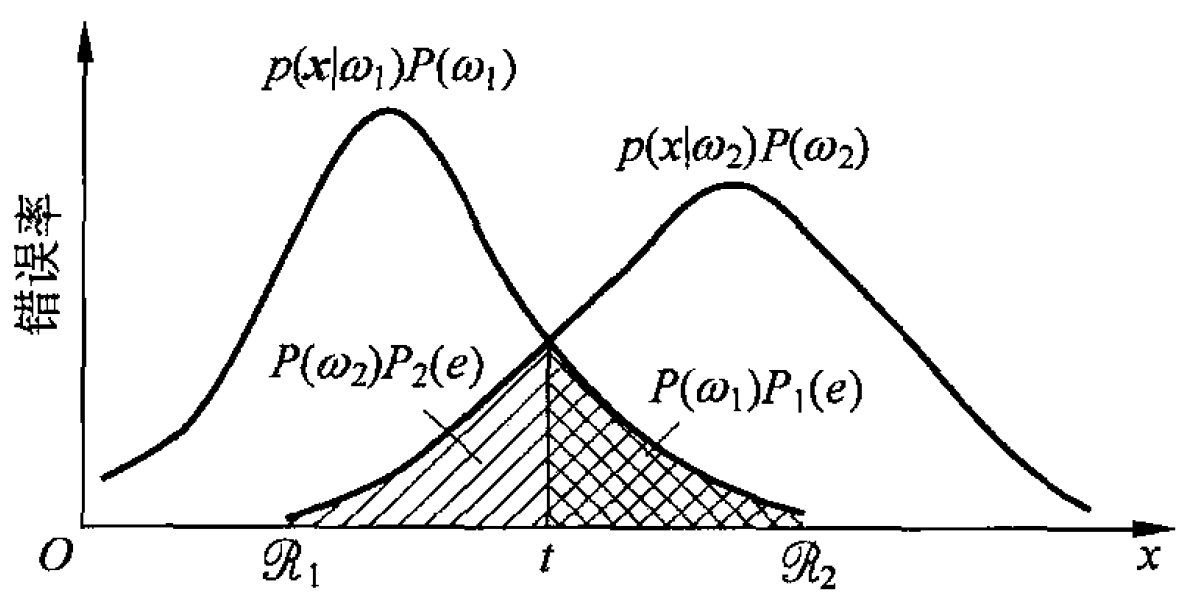
\includegraphics[width=8cm]{1627807965262-1.2.png}
  \caption{错误率计算图示[1]}
\end{figure}

多类错误率:通过平均正确率来计算平均错误率

\begin{equation}
\begin{aligned}
  P\left(c \right)
  &=\sum_{j=1}^c{P\left(x\in \mathcal{R}_j|\omega_j \right)P\left(\omega_j \right)}\\
  &=\sum_{j=1}^c{\int_{\mathcal{R}_j}{p\left(x|\omega_j \right)P\left(\omega_j \right)}}\mathrm{d}x
\end{aligned}
\end{equation}

\begin{equation}
\begin{aligned}
  P\left(e \right)
  &=\sum_{i=1}^c{\sum_{j\ne i}{P\left(x\in \mathcal{R}_j|\omega_i \right)P\left(\omega_i \right)}}\\
  &=1-P\left(c \right)
\end{aligned}
\end{equation}

\section{最小风险贝叶斯决策}

基本思想:不同的决策错误所带来的损失可能不同

决策论表述:样本 $x\in\mathbb{R}^d$ 看做随机向量

状态空间:$c$ 个可能的状态 (类别) 

\begin{equation}
\Omega =\left\{ \omega_1,\omega_2,\dots ,\omega_c \right\}
\end{equation}

决策空间:判定样本为某类或拒绝等

\begin{equation}
\mathcal{A} =\left\{ \alpha_1,\alpha_2,\dots ,\alpha_k \right\}
\end{equation}

一般 $k\geqslant c$,

\begin{equation}
\alpha_i=\left\{ x\in \omega_i \right\} , i=1,\dots ,c
\end{equation}

$\alpha_{c+1}=\mathrm{reject}$ 等

损失函数:实际为 $\omega_j$ 类判定为 $\alpha_i$ 的损失 $\lambda \left(\alpha_i,\omega_j \right)$ →决策表

期望损失:

\begin{equation}
\begin{aligned}
  R\left(\alpha_i|x \right)
  &=\mathbb{E} \left[\lambda \left(\alpha_i,\omega_j \right)|x \right]\\
  &=\sum_j\lambda \left(\alpha_i,\omega_j \right)P\left(\omega_j|x \right)
\end{aligned}
\end{equation}

期望风险:

\begin{equation}
R\left(\alpha \right)=\int_{-\infty}^{\infty}{R\left(\alpha |x \right)p(x)}\mathrm{d}x
\end{equation}

最小风险决策:

\begin{equation}
\min R\left(\alpha \right)\Rightarrow \alpha =\mathrm{argmin}_jR\left(\alpha_j|x \right)
\end{equation}

与最小错误率决策等价:0-1 决策表

\begin{equation}
\lambda \left(\alpha_i,\omega_j \right)=1-\delta_{ij}
\end{equation}

则

\begin{equation}
\begin{aligned}
  R\left(\alpha_i|x \right)
  &=\sum_j\lambda \left(\alpha_i,\omega_j \right)P\left(\omega_j|x \right)\\
  &=\sum_{j\ne i}P\left(\omega_j|x \right)\\
  &=1-P\left(\omega_i|x \right)
\end{aligned}
\end{equation}

因此

\begin{equation}
\begin{aligned}
  \min R\left(\alpha \right)
  &\Rightarrow \min_jR\left(\alpha_j|x \right)\\
  &\Rightarrow \alpha =\mathrm{argmax}_jP\left(\omega_j|x \right)
\end{aligned}
\end{equation}

似然比:

\begin{equation}
l(x)=\frac{P\left(x|\omega_1 \right)}{P\left(x|\omega_2 \right)}>\frac{P\left(\omega_2 \right)}{P\left(\omega_1 \right)}\frac{\lambda_{12}-\lambda_{22}}{\lambda_{21}-\lambda_{11}}\Rightarrow x\in \omega_1
\end{equation}

\section{限定一类错误率条件下使另一类错误率最小}

Neyman-Pearson 决策:优化问题

\begin{equation}
\min \left\{ P_1\left(e \right)|P_2\left(e \right)-\epsilon_0=0 \right\}
\end{equation}

\begin{equation}
\begin{aligned}
  L
  &=P_1\left(e \right)+\lambda \left(P_2\left(e \right)-\epsilon_0 \right)\\
  &=\int_{\mathcal{R}_2}{p\left(x|\omega_1 \right)}\mathrm{d}x+\lambda \left(\int_{\mathcal{R}_1}{p\left(x|\omega_2 \right)}\mathrm{d}x-\epsilon_0 \right)\\
  &=1-\lambda \epsilon_o+\int_{\mathcal{R}_1}{\left[\lambda p\left(x|\omega_2 \right)-p\left(x|\omega_1 \right)\right]}\mathrm{d}x
\end{aligned}
\end{equation}

梯度条件:决策边界满足

\begin{equation}
\lambda =\frac{p\left(x|\omega_1 \right)}{p\left(x|\omega_2 \right)},~P_2\left(e \right)=\epsilon_0
\end{equation}

决策规则:

\begin{equation}
\lambda p\left(x|\omega_2 \right)-p\left(x|\omega_1 \right)<0\Rightarrow x\in \omega_1
\end{equation}

似然比:

\begin{equation}
l(x)=\frac{p\left(x|\omega_1 \right)}{p\left(x|\omega_2 \right)}>\lambda \Rightarrow x\in \omega_1
\end{equation}

对偶变量求解:通过 $l(x)$ 的映射关系,可由 $p(x)$ 求得 $p\left(l|\omega_2 \right)$,则由定义可知误差率为

\begin{equation}
\begin{aligned}
  P_2\left(e \right)
  &=1-\int_0^{\lambda}{p\left(l|\omega_2 \right)\mathrm{d}l}\\
  &=\epsilon_0\Rightarrow \lambda
\end{aligned}
\end{equation}

\section{朴素贝叶斯}

随机向量分量独立:

\begin{equation}
p\left(\vec{x}|\omega \right)=p\left(x_1,\dots ,x_d|\omega \right):=\prod_ip\left(x_i|\omega \right)
\end{equation}

\section{判别函数与正态分布}

判别函数:$g_i(x)$,例如后验概率

\begin{equation}
g_i(x)=P\left(\omega_i|x \right)
\end{equation}

取分子

\begin{equation}
g_i(x)=p\left(x|\omega_i \right)P\left(\omega_i \right)
\end{equation}

取对数

\begin{equation}
g_i(x)=\ln p\left(x|\omega_i \right)+\ln P\left(\omega_i \right)
\end{equation}

决策面方程:$g_i(x)=g_j(x)$

正态分布:

\begin{equation}
p(x)=\frac{1}{\left(2\pi \right)^{d/2}|\Sigma |^{1/2}}\exp \left\{ -\frac{1}{2}\left(x-\mu \right)^{\top}\Sigma ^{-1}\left(x-\mu \right)\right\}
\end{equation}

维数 $d$,均值 $\mu =\mathbb{E} \left[x \right]$,协方差

\begin{equation}
\Sigma =\mathbb{E} \left[\left(x-\mu \right)\left(x-\mu \right)^{\top} \right]
\end{equation}

贝叶斯判别:各类分布

\begin{equation}
p\left(x|\omega_i \right)\sim \mathcal{N} \left(\mu_i,\Sigma_i \right)
\end{equation}

则判别函数为

\begin{equation}
g_i(x)=-\frac{d}{2}\ln 2\pi -\frac{1}{2}\ln |\Sigma_i|+\ln P\left(\omega_i \right)-\frac{1}{2}\left(x-\mu_i \right)^{\top}\Sigma_{i}^{-1}\left(x-\mu_i \right)
\end{equation}

决策面方程:$g_i(x)=g_j(x)$,即

\begin{equation}
\begin{aligned}
  &-0.5\left[\left(x-\mu_i \right)^{\top}\Sigma_{i}^{-1}\left(x-\mu_i \right)-\left(x-\mu_j \right)^{\top}\Sigma_{j}^{-1}\left(x-\mu_j \right)\right]\\
  &+\left[\ln P\left(\omega_i \right)-\ln P\left(\omega_j \right)\right] -0.5\left(\ln |\Sigma_i|-\ln |\Sigma_j| \right)=0
\end{aligned}
\end{equation}

\section{分类性能评价 ROC 与 AUC}

ROC (Receiver Operating Characteristic):FP-TP 曲线,越靠近曲线左上角的点对应的阈值参数性能越好

混淆矩阵:两类分类问题

\begin{table}
  \centering
  \begin{tabular}{ccc}
    \hline
           & 实际为正类 & 实际为负类   \\ \hline
     预测为正类 & TP    & FP     \\
     预测为负类 & FN    & TN     \\ \hline
  \end{tabular}
\end{table}

AUC (Area Under ROC Curves):ROC 曲线下方面积越大越好

例:给定样本标签 

\begin{equation}
y = [1~0~1~1~1~0~0~0]
\end{equation}

分类器输出结果为

\begin{equation}
S = [0.5~0.3~0.6~0.22~0.4~0.51~0.2~0.33]
\end{equation}

则 FP 与 TP 计算如下:

\begin{table}
  \centering
  \begin{tabular}{cccc}
    \hline
    class & score & FP   & TP   \\
    \hline
    1     & 0.6   & 0    & 0.25 \\
    0     & 0.51  & 0.25 & 0.25 \\
    1     & 0.5   & 0.25 & 0.5  \\
    1     & 0.4   & 0.25 & 0.75 \\
    1     & 0.33  & 0.5  & 0.75 \\
    0     & 0.3   & 0.75 & 0.75 \\
    0     & 0.22  & 0.75 & 1    \\
    0     & 0.2   & 0.1  & 1   \\
    \hline
  \end{tabular}
\end{table}

\begin{figure}
  \centering
  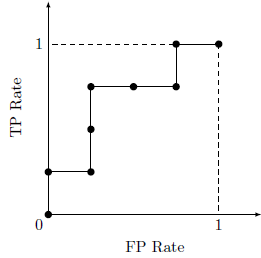
\includegraphics[width=6cm]{1627808143710-1.7.png}
  \caption{ROC 曲线}
\end{figure}

\chapter{概率密度函数估计}

统计量:样本的分布信息,如均值,方差等

参数空间:未知参数向量 $\theta$ 全部可能取值的集合 $\Theta$

点估计:构造估计量 $d\left(x_1,\dots ,x_N \right)$ 作为 $\theta$ 的估计

区间估计:构造置信区间 $\left(d_1,d_2 \right)$ 作为 $\theta$ 可能取值范围的估计

\section{极大似然估计 (MLE, Maximum Likelihood Estimate) }

假设:

1. 概率分布函数形式已知

2. 样本独立同分布采样得到

似然函数:

\begin{equation}
\begin{aligned}
  l(\theta)
  &=p(X|\theta)\\
  &=p(x_1,\dots ,x_N|\theta)\\
  &=\prod_kp(x_k|\theta)
\end{aligned}
\end{equation}

对数似然函数:

\begin{equation}
\begin{aligned}
  H(\theta)
  &=\ln l(\theta)\\
  &=\sum_k\ln p(x_k|\theta)
\end{aligned}
\end{equation}

极大似然估计:

\begin{equation}
\begin{aligned}
  \theta 
  &=\mathrm{argmax}_{\theta\in\Theta} l(\theta)\\
  &=\mathrm{argmax}_{\theta\in\Theta} H(\theta)
\end{aligned}
\end{equation}

正态分布:待估计参数为 $\theta=[\mu,\sigma^2]$, 数据点 

\begin{equation}
X=\{ x_1,\dots,x_N\}
\end{equation}

估计量为 $\hat{\theta}=[\hat{\mu},\hat{\sigma}^2]$

概率密度函数为

\begin{equation}
p(x_k|\theta)=\frac{1}{\sqrt{2\pi}\sigma}\exp \left[-\frac{(x_k-\mu)^2}{2\sigma^2} \right]
\end{equation}

取对数得

\begin{equation}
\ln p(x_k|\theta)=-\frac{1}{2}\ln \left(2\pi \theta_2 \right)-\frac{\left(x_k-\theta_1 \right)^2}{2\theta_2}
\end{equation}

对 $\theta$ 求梯度有

\begin{equation}
\nabla_{\theta}\ln p(x_k|\theta)
=\begin{bmatrix}
  \dfrac{x_k-\theta_1}{\theta_2}\\ 
  -\dfrac{1}{2\theta_2}+\dfrac{\left(x_k-\theta_1 \right)^2}{2\theta_{2}^{2}}\\
\end{bmatrix}
\end{equation}

又

\begin{equation}
\sum_{k=1}^N{\nabla_{\theta}\ln p(x_k|\theta)}=0
\end{equation}

因此,估计量为
\begin{equation}
\begin{aligned}
  \hat{\mu}&=\frac{1}{N}\sum_{k=1}^N{x_k} \\
  \hat{\sigma}^2&=\frac{1}{N}\sum_{k=1}^N{\left(x_k-\hat{\mu} \right)^2}
\end{aligned}
\end{equation}

多元正态分布:

\begin{equation}
\begin{aligned}
  \hat{\mu}&=\frac{1}{N}\sum_{k=1}^N{x_k}\\
  \hat{\Sigma}&=\frac{1}{N}\sum_{k=1}^N{\left(x_k-\hat{\mu} \right)\left(x_k-\hat{\mu} \right)^{\top}}
\end{aligned}
\end{equation}

无偏估计:

\begin{equation}
\mathbb{E} \left[\hat{\mu} \right] =\mu
\end{equation}

\begin{equation}
\mathbb{E} \left[\frac{N}{N-1}\hat{\Sigma}\right] =\Sigma
\end{equation}

渐进无偏估计:

\begin{equation}
\lim_{n\rightarrow \infty} \mathbb{E} \left[\hat{\Sigma} \right] =\Sigma
\end{equation}

可识别性:对 $\theta \ne \theta '$, 

\begin{equation}
\exists~x\Rightarrow p(X|\theta)\ne p\left(x|\theta ' \right)
\end{equation}

离散随机变量的混合密度函数往往不可识别,连续的则一般可以识别

\section{贝叶斯估计}

假设:参数 $\theta$ 是随机变量,且已知其先验分布 $p(\theta)$

贝叶斯估计:后验概率

\begin{equation}
p\left(\theta |X \right)=p(X|\theta)p(\theta)/p(x)
\end{equation}

贝叶斯学习:

\begin{equation}
\begin{aligned}
  p\left(x|X \right)
  &=\int{p\left(x,\theta |X \right)\mathrm{d}\theta}\\
  &=\int{p(X|\theta)p\left(\theta |X \right)\mathrm{d}\theta}
\end{aligned}
\end{equation}

贝叶斯学习性质:

\begin{equation}
\lim_{N\rightarrow \infty} p\left(x|X^N \right)=p\left(x|\hat{\theta}=\theta \right)=p(x)
\end{equation}

正态分布:

\begin{equation}
p(X|\mu)\sim \mathcal{N} \left(\mu ,\sigma^2 \right)
\end{equation}

\begin{equation}
p(\mu)\sim \mathcal{N} \left(\mu_o,\sigma_{0}^{2} \right)
\end{equation}

其中 $\sigma^2$ 已知,则有

\begin{equation}
\begin{aligned}
  p(\mu|X)
  &=\frac{p(X|\mu)p(\mu)}{p(x)}\\
  &=\alpha \prod_kp\left(x_k|\mu \right)p(\mu)\\
  &=\alpha '\cdot \exp \left\{ -\frac{1}{2}\left[\sum_{k=1}^N{\frac{\left(\mu -x_k \right)^2}{\sigma^2}}+\frac{\left(\mu -\mu_0 \right)^2}{\sigma_{0}^{2}} \right] \right\} \\
  &:=\frac{1}{\sqrt{2\pi}\sigma_N}\exp \left[-\frac{\left(\mu -\mu_N \right)^2}{2\sigma_{N}^{2}} \right]
\end{aligned}
\end{equation}

其中

\begin{equation}
\sigma_{N}^{2}=\frac{\sigma_{0}^{2}\sigma^2}{N\sigma_{0}^{2}+\sigma^2}
\end{equation}

\begin{equation}
\mu_N=\frac{N\sigma_{0}^{2}}{N\sigma_{0}^{2}+\sigma^2}m_N+\frac{\sigma^2}{N\sigma_{0}^{2}+\sigma^2}\mu_0
\end{equation}

其中

\begin{equation}
m_N=\frac{1}{N}\sum_{k=1}^N{x_k}
\end{equation}

因此

\begin{equation}
\begin{aligned}
  p\left(x|X \right)
  &=\int{p(X|\mu)p(\mu|X)\mathrm{d}\mu}\\
  &\sim \mathcal{N} \left(\mu_N,\sigma^2+\sigma_{N}^{2} \right)
\end{aligned}
\end{equation}

参数变化:

\begin{equation}
\sigma_0=0\Rightarrow \mu_N=\mu_0
\end{equation}

\begin{equation}
N\uparrow \Rightarrow \mu_N\rightarrow m_N,~\sigma_{N}^{2}\rightarrow 0
\end{equation}

最大似然估计与贝叶斯估计对比:

1. 训练样本无穷多时,最大似然估计与贝叶斯估计结果相同

2. 贝叶斯估计使用先验概率利用了更多信息,若信息可靠则贝叶斯估计更准确,但有时先验概率很难设计,无信息先验

3. 最大似然估计计算简单,贝叶斯通常计算复杂的积分

4. 最大似然估计易于理解,给出的是参数的最佳估计结果

\section{非参数估计}

假设:

1. 概率分布函数形式未知

2. 样本独立同分布

直方图估计:

\begin{equation}
\hat{p}_N(x)
=\frac{k_N}{NV_N}
\rightarrow p(x)
\end{equation}

估计收敛条件:

\begin{equation}
V_N\rightarrow 0,~k_N\rightarrow \infty ,~k_N/N\rightarrow 0
\end{equation}

\section{Parzen 窗估计 (Kernel Density Estimation) }

思想:固定小舱体积,滑动小舱估计每个点的概率密度

区域:$R_N$ 是 $d$ 维超立方体,棱长 $h_N$,体积 $V_N=h_{N}^{d}$

窗函数条件:$\displaystyle\phi \left(u \right)\geqslant 0,~\int{\phi \left(u \right)\mathrm{d}u}=1$

1. 方窗:
  \begin{equation}
  \phi \left(u \right)=
  \begin{cases}
    1, &\mathrm{if}~\left\| u \right\|_{\infty}\leqslant 1/2\\
    0, &\mathrm{otherwise}
  \end{cases}
  \end{equation}
2. 正态窗:
  \begin{equation}
  \phi \left(u \right)=\frac{1}{\sqrt{2\pi}}\exp \left(-\frac{1}{2}u^2 \right),~u\in\mathbb{R}
  \end{equation}
3. 指数窗:
  \begin{equation}
  \phi \left(u \right)=\frac{1}{2}\exp \left(-|u| \right),~u\in\mathbb{R}
  \end{equation}

落入以 $x$ 为中心的区域的样本数:

\begin{equation}
k_N=\sum_{i=1}^N{\phi \left(\frac{x-x_i}{h_N} \right)}
\end{equation}

概率密度函数估计:

\begin{equation}
\hat{p}_N(x)=\frac{1}{N}\sum_{i=1}^N{\frac{1}{V_N}\phi \left(\frac{x-x_i}{h_N} \right)}
\end{equation}

窗宽选取:$h_N=h_1/\sqrt{N}$,其中 $h_1$ 可调且一般存在最优值

估计量性质:一维正态窗

\begin{equation}
\begin{aligned}
  \bar{p}_N
  &=\mathbb{E} \left[\hat{p}_N(x)\right] \\
  &\sim \mathcal{N} \left(\mu ,\sigma^2+h_{N}^{2} \right)
\end{aligned}
\end{equation}

\section{\texorpdfstring{$k_N$}{kN} 近邻估计}

思想:固定小舱内数据点个数,滑动可变大小的小舱对每个采样点 (而不是数据点) 进行概率密度估计

数据点个数:$k_N=k_1\sqrt{N}$,其中 $k_1$ 可调且一般存在最优值

\section{估计准确性、维数问题与过拟合}

估计准确性:

1. 贝叶斯误差:不同的类条件概率分布函数之间的相互重叠

2. 模型误差:选择了错误的概率密度函数模型

3. 估计误差:采用有限样本进行估计所带来的误差

维数问题:维数为 $d$,需要样本 $100^d$ →维数灾难

过拟合避免方法:

1. 贝叶斯方法

2. 增加样本数

3. 正则化

4. 减少模型参数

\chapter{EM 算法与高斯混合模型 GMM}

\section{EM 算法}

思想:用隐变量对缺失数据建模,迭代实现最大似然估计

数据:$X=\{ x_1,\dots,x_N\}$,隐变量 $Y$,完整数据 $Z=\left(X,Y \right)$

似然函数:

\begin{equation}
\begin{aligned}
  l(\theta)
  &=p(X|\theta)\\
  &=\sum_{y\in Y}p\left(X,y|\theta \right)
\end{aligned}
\end{equation}

对数似然函数:

\begin{equation}
\begin{aligned}
  L(\theta)
  &=\ln l(\theta)\\
  &=\ln \sum_{y\in Y}p\left(X,y|\theta \right)
\end{aligned}
\end{equation}

对数似然函数的下界:应用 Jensen 不等式于对数函数可得

\begin{equation}
\begin{aligned}
  L(\theta)
  &=\ln \sum_yp\left(X,y|\theta \right)\\
  &=\ln \sum_y\frac{q(y)p\left(X,y|\theta \right)}{q(y)}\\
  &\geqslant \sum_yq(y)\ln\frac{p\left(X,y|\theta \right)}{q(y)} \\
  &=\sum_yq(y)\ln p\left(X,y|\theta \right)-\sum_yq(y)\ln q(y)\\
  &:=F\left(q,\theta \right)
\end{aligned}
\end{equation}

迭代优化下界:初始化 $q_{\left[0 \right]},~\theta_{\left[0 \right]}$ 后反复迭代

\begin{equation}
\begin{aligned}
  q_{\left[k+1 \right]}&\gets \mathrm{argmax}_qF\left(q,\theta_{\left[k \right]} \right)\\
  \theta_{\left[k+1 \right]}&\gets \mathrm{argmax}_{\theta}F\left(q_{\left[k+1 \right]},\theta \right)
\end{aligned}
\end{equation}

\begin{figure}
  \centering
  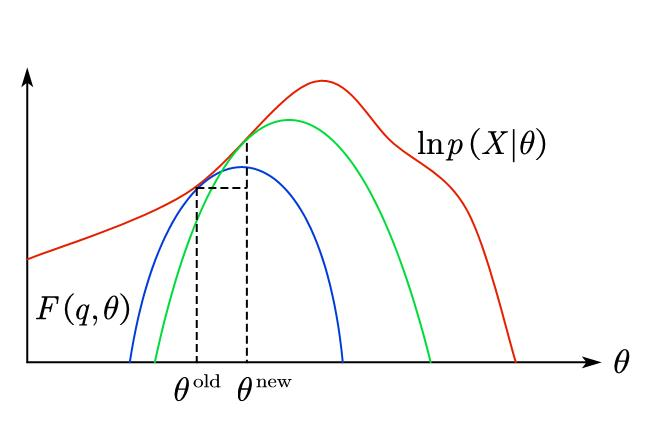
\includegraphics[width=8cm]{1627808293080-3.1.jpg}
  \caption{迭代优化下界}
\end{figure}

期望:当 $q=p\left(y|X,\theta_{\left[k \right]} \right)$ 为后验概率时,$F\left(q,\theta_{\left[k \right]} \right)$ 达到最大

\begin{equation}
\begin{aligned}
  F\left(q,\theta \right)
  &=\sum_yq(y)\ln\frac{p\left(X,y|\theta \right)}{q(y)}\\
  &=\sum_yp\left(y|X,\theta \right)\ln\frac{p\left(y|X,\theta \right)p(X|\theta)}{p\left(y|X,\theta \right)} \\
  &=\sum_yp\left(y|X,\theta \right)\ln p(X|\theta)\\
  &=\ln p(X|\theta)\\
  &=L(\theta)
\end{aligned}
\end{equation}

\begin{equation}
\begin{aligned}
  F\left(q_{\left[k+1 \right]},\theta \right)=\sum_yq_{\left[k+1 \right]}(y)\ln p\left(X,y|\theta \right)-\sum_yq_{\left[k+1 \right]}(y)\ln q_{\left[k+1 \right]}(y)
\end{aligned}
\end{equation}

第二项不包含优化变量 $\theta$ 可忽略,代入 $q_{\left[k+1 \right]}(y)$ 并定义

\begin{equation}
\begin{aligned}
  Q\left(\theta_{\left[k \right]},\theta \right)&:=\sum_yp\left(y|X,\theta_{\left[k \right]} \right)\ln p\left(X,y|\theta \right)\\
  &=\mathbb{E} \left[\ln p\left(X,y|\theta \right)|X,\theta_{\left[ k \right]} \right]
\end{aligned}
\end{equation}

最大化:

\begin{equation}
\theta_{\left[k+1 \right]}\gets \mathrm{argmax}_{\theta}Q\left(\theta_{\left[k \right]},\theta \right)
\end{equation}

广义最大化:

\begin{equation}
\theta_{\left[k+1 \right]}\in \left\{ \theta_{\left[k+1 \right]}|Q\left(\theta_{\left[k \right]},\theta_{\left[k+1 \right]} \right)>Q\left(\theta_{\left[k \right]},\theta_{\left[k \right]} \right)\right\}
\end{equation}

\section{高斯混合模型 GMM}

隐变量:$Y=\left\{ y\in \mathbb{R} ^N \right\}$ 表示样本 $x_i$ 由第 $y_i$ 个高斯分布产生

混合模型:

\begin{equation}
p(X|\theta)=\Sigma_j\alpha_jp_j\left(X|\theta_j \right)
\end{equation}

其中

\begin{equation}
\Theta =\left\{ \alpha_j,\theta_j \right\},~\sum_j\alpha_j=1
\end{equation}

由独立同分布可得

\begin{equation}
\begin{aligned}
  p(X|\theta)
  &=\prod_ip\left(x_i|\Theta \right)\\
  &=\prod_i\sum_j\alpha_jp_j\left(x_i|\theta_j \right)
\end{aligned}
\end{equation}

对数似然函数:

\begin{equation}
\ln p(X|\theta)=\sum_i\ln \sum_j\alpha_jp_j\left(x_i|\theta_j \right)
\end{equation}

极大似然估计:

\begin{equation}
\nabla_{\Theta}\ln p(X|\theta)=0\Rightarrow \Theta
\end{equation}

结果与EM相同

EM 算法:

\begin{equation}
p\left(X,y|\Theta \right)=\prod_ip\left(x_i|y_i \right)p\left(y_i \right)
\end{equation}

\begin{equation}
\begin{aligned}
  \ln p\left(X,y|\Theta \right)
  &=\sum_i\ln p\left(x_i|y_i \right)p\left(y_i \right)\\
  &=\sum_i\ln \alpha_{y_i}p_{y_i}\left(x_i|\theta_{y_i} \right)
\end{aligned}
\end{equation}

\begin{equation}
\begin{aligned}
  p\left(y|X,\Theta ^g \right)
  &=\prod_ip\left(y_i|x_i,\Theta ^g \right)\\
  &=\prod_i\alpha_{y_i}^{g}\frac{p_{y_i}\left(x_i|\theta_{y_i}^{g} \right)}{p\left(x_i|\Theta ^g \right)}
\end{aligned}
\end{equation}

\begin{equation}
\begin{aligned}
  Q\left(\Theta ^g,\Theta \right)
  &=\sum_yp\left(y|X,\Theta ^g \right)\ln p\left(X,y|\Theta \right)\\
  &=\sum_j\sum_i\ln \left(\alpha_jp_j\left(x_i|\theta_j \right)\right)p\left(j|x_i,\Theta ^g \right)\\
  &=\sum_j\sum_ip\left(j|x_i,\Theta ^g \right)\left[\ln \alpha_j+\ln p_j\left(x_i|\theta_j \right)\right]
\end{aligned}
\end{equation}

$\alpha_j$ 与 $\theta_j$ 解耦可分别优化,由 $\sum_i\alpha_i=1$ 及梯度条件解得

\begin{equation}
\begin{aligned}
  \alpha_{j}^{\mathrm{new}}&=\frac{1}{N}\sum_ip\left(j|x_i,\Theta ^g \right)\\ 
  \mu_{j}^{\mathrm{new}}&=\frac{1}{N\alpha_{j}^{\mathrm{new}}}\sum_ix_ip\left(j|x_i,\Theta ^g \right)\\
  \Sigma_{j}^{\mathrm{new}}&=\frac{1}{N\alpha_{j}^{\mathrm{new}}}\sum_ip\left(j|x_i,\Theta ^g \right)\left(x_i-\mu_{j}^{\mathrm{new}} \right)\left(x_i-\mu_{j}^{\mathrm{new}} \right)^{\top}
\end{aligned}
\end{equation}

若限制各成分的协方差矩阵均相同,则 M 步需要修改为

\begin{equation}
\Sigma ^{\mathrm{new}}=\sum_{j}\sum_i\frac{p\left(j|x_i,\Theta ^g \right)\left(x_i-\mu_{j}^{\mathrm{new}} \right)\left(x_i-\mu_{j}^{\mathrm{new}} \right)^{\top}}{N\sum_j\alpha_{j}^{\mathrm{new}}}
\end{equation}

例题:三维数据点,偶数点的第3维数据缺失,令 $x_{i3},~i\in E$ 为隐变量,

\begin{equation}
x_i=\left[x_{i1},x_{i2},x_{i3} \right] ^{\top}
\end{equation}

则对数似然函数为

\begin{equation}
\begin{aligned}
  L(\theta)
  &=\sum_{i\in O}\ln p\left(x_{i1},x_{i2},x_{i3}|\theta \right)+\sum_{i\in E}\ln p\left(x_{i1},x_{i2}|\theta \right)\\
  &=\sim +\sum_{i\in E}\ln \int_{-\infty}^{+\infty}p\left(x_{i1},x_{i2},x_{i3}|\theta \right)\mathrm{d}x_{i3}\\
  &=\sim +\sum_{i\in E}\ln \int_{-\infty}^{+\infty}\frac{q\left(x_{i3} \right)p\left(x_{i1},x_{i2},x_{i3}|\theta \right)}{q\left(x_{i3} \right)}\mathrm{d}x_{i3}\\
  &\geqslant \sim +\sum_{i\in E}\int_{-\infty}^{+\infty}q\left(x_{i3} \right)\ln\frac{p\left(x_{i1},x_{i2},x_{i3}|\theta \right)}{q\left(x_{i3} \right)} \mathrm{d}x_{i3}
\end{aligned}
\end{equation}

\begin{equation}
Q\left(\theta_{\left[k \right]},\theta \right)=\sim +\sum_{i\in E}\int_{-\infty}^{+\infty}p\left(x_{i3}|x_{i1},x_{i2},\theta_{\left[k \right]} \right)\ln p\left(\vec{x}_i|\theta \right)\mathrm{d}x_{i3}
\end{equation}

\chapter{线性判别函数}

思想:

1. 不恢复类条件概率密度,利用样本直接设计分类器

2. 线性判别函数形式简单易分析,但往往不是最优分类器

线性判别函数:$g(x)=w^{\top}x+w_0$

两类问题:$g(x)=g_1(x)-g_2(x)$,分类决策为

\begin{equation}
\begin{cases}
  x\in \omega_1, &\mathrm{if}~g(x)>0\\
  x\in \omega_2, &\mathrm{if}~g(x)<0\\
  \mathrm{either}~\mathrm{or}~\mathrm{reject}, &\mathrm{otherwise}
\end{cases}
\end{equation}

点到直线距离:

\begin{equation}
r=\frac{g(x)}{\left\| w \right\|}
\end{equation}

广义线性判别:

\begin{equation}
g(x)=w^{\top}x+w_0:=a^{\top}y
\end{equation}

其中增广样本向量为 

\begin{equation}
y=\begin{bmatrix}
  1\\ x
\end{bmatrix}
\end{equation}

增广权向量为 

\begin{equation}
a=\begin{bmatrix}
  w_0\\ w
\end{bmatrix}
\end{equation}

样本规范化:

\begin{equation}
y_{i}'=
\begin{cases}
  y_i, & \mathrm{if}~y_i\in \omega_1\\
  -y_i, & \mathrm{if}~y_i\in \omega_2
\end{cases}
\end{equation}

解区:解向量集合 $\left\{ a|a^{\top}y_{i}'>0,~\forall~i \right\}$

解区限制:$a^{\top}y_i\geqslant b>0,~\forall~i$

感知准则函数:

\begin{equation}
\min J_p\left(a \right)=\sum_{y\in Y^k}\left(-a^{\top}y \right)
\end{equation}

最小化错分样本 $y\in Y^k$ 到分界面距离之和,梯度为

\begin{equation}
\nabla J_p\left(a \right)=\sum_{y\in Y^k}\left(-y \right)
\end{equation}

迭代公式为

\begin{equation}
a\left(k+1 \right)=a\left(k \right)+\rho_k\sum_{y\in Y^k}y
\end{equation}

直到 $a$ 不变

单样本感知器算法:循环处理每个样本,若 $a^{\top}y^k\leqslant \gamma$,其中 $\gamma \geqslant 0$,则 

\begin{equation}
a\left(k+1 \right)=a\left(k \right)+y^k
\end{equation}

直到所有样本满足条件

多类问题:

1. $c-1$ 个非己:$\omega_1$ 与非 $\omega_1$,$\omega_2$ 与非 $\omega_2$,双非为 $\omega_3$

2. $c\left(c-1 \right)/2$ 个两类:$\omega_1-\omega_2$, $\omega_1-\omega_3$, $\omega_2-\omega_3$ 三条线

3. 直接设计判别函数:
\begin{equation}
  \mathcal{R}_i=\left\{ x|g_i(x)>g_j(x),~\forall~j\ne i \right\}
\end{equation}

\chapter{支持向量机SVM}

判别式模型:直接利用样本计算判别函数

\section{线性可分情形}

样本集合:

\begin{equation}
  T=\left\{ \left(x_i,y_i \right)\right\}_{i=1}^{N}
\end{equation}

其中

\begin{equation}
  y_i=
  \begin{cases}
    1, &\mathrm{if}~x_i\in \omega_1\\
    -1, &\mathrm{if}~x_i\in \omega_2\\
  \end{cases}
\end{equation}

线性判别函数:

\begin{equation}
  y_i\left(w^{\top}x_i+b \right)\geqslant 1,~\forall~i
\end{equation}

margin 

\begin{equation}
  \rho=\frac{2}{\|w\|}
\end{equation}

优化问题:

\begin{equation}
  \min \left\{\frac{1}{2}w^{\top}w|y_i\left(w^{\top}x_i+b \right)\geqslant 1, i=1,\dots ,N \right\}
\end{equation}

Lagrange 函数为

\begin{equation}
  L\left(w,b,\alpha \right)=\frac{1}{2}w^{\top}w-\sum_{i=1}^{N}\alpha_i\left[y_i\left(w^{\top}x_i+b \right)-1 \right]
\end{equation}

梯度条件:

\begin{equation}
  w=\sum_{i=1}^{N}\alpha_iy_ix_i,~\sum_{i=1}^{N}\alpha_iy_i=0
\end{equation}

对偶函数:

\begin{equation}
  Q\left(\alpha \right)=\sum_{i=1}^{N}\alpha_i-\frac{1}{2}\sum_{i=1}^{N}\sum_{j=1}^{N}\alpha_i\alpha_jy_iy_jx_{i}^{\top}x_j
\end{equation}

对偶问题:

\begin{equation}
  \max \left\{ Q\left(\alpha \right)|\sum_{i=1}^{N}\alpha_iy_i=0,~\alpha \geqslant 0 \right\}
\end{equation}

支持向量:互补松弛

\begin{equation}
  \alpha_{i}^{*}\left[y_i\left(\left< w^*,x_i \right> +b \right)-1 \right] =0,~\alpha_{i}^{*}\ne 0
\end{equation}

支持向量机:

\begin{equation}
  f(x)=\mathrm{sgn} \left(\sum_i\alpha_{i}^{*}y_ix_{i}^{\top}x+b^* \right)\in \left\{ -1,+1 \right\}
\end{equation}

\section{线性不可分情形}

Soft margin:$y_i\left(w^{\top}x_i+b \right)\geqslant 1-\xi_i,~\forall~i$

松弛变量:

\begin{equation}
  \begin{cases}
    0\leqslant \xi_i\leqslant 1, &\mathrm{if}~\mathrm{violated}\\
    \xi_i>1, &\mathrm{if}~\mathrm{misclassified}
  \end{cases}
\end{equation}

优化问题:错分率上界 $\sum_i\xi_i$,tradeoff $C$

\begin{equation}
  \begin{aligned}
    \min~~&\frac{1}{2}w^{\top}w+C\sum_i\xi_i\\
    \mathrm{s.t.}~~& y_i\left(w^{\top}x_i+b \right)\geqslant 1-\xi_i,~\forall~i\\
    &\xi_i\geqslant 0,~\forall~i
  \end{aligned}
\end{equation}

无约束形式:

\begin{equation}
  \min~\frac{1}{2}w^{\top}w+C\sum_iL\left(w,b;x_i,y_i \right)
\end{equation}

其中 Hinge 损失函数为

\begin{equation}
  L\left(w,b;x_i,y_i \right)=\max \left\{ 1-y_i\left(w^{\top}x_i+b \right),0 \right\}
\end{equation}

对偶问题:

\begin{equation}
  \max \left\{ Q\left(\alpha \right)|\sum_{i=1}^{N}\alpha_iy_i=0,~0\leqslant \alpha \leqslant C \right\}
\end{equation}

\section{非线性情形 Kernel SVM}

广义线性可分:低维空间 $L$ 升到高维空间 $H$ 使样本线性可分

升维原因:输入空间 $L$ 一般不是正常的特征空间

核函数:

\begin{equation}
  K\left(x_i,x_j \right)=\left< \Phi \left(x_i \right),\Phi \left(x_j \right)\right>
\end{equation}

其中 $\Phi :L\rightarrow H$

多项式核函数:

\begin{equation}
  K\left(x,y \right)=\left(\gamma \left< x,y \right> +r \right)^p, \gamma >0
\end{equation}

径向基 RBF 核函数:

\begin{equation}
  K\left(x,y \right)=\exp \left(-\frac{\left\| x-y \right\|^2}{2\sigma^2}\right)
\end{equation}

Sigmiod 核函数:

\begin{equation}
  K\left(x,y \right)=\tanh \left(\kappa \left< x,y \right> -\delta \right)
\end{equation}

对偶函数:

\begin{equation}
  Q\left(\alpha \right)=\sum_{i=1}^{N}\alpha_i-\frac{1}{2}\sum_{i=1}^{N}\sum_{j=1}^{N}\alpha_i\alpha_jy_iy_jK\left(x_i,x_j \right)
\end{equation}

对偶问题:

\begin{equation}
  \max \left\{ Q\left(\alpha \right)|\sum_{i=1}^{N}\alpha_iy_i=0,~0\leqslant \alpha \leqslant C \right\}
\end{equation}

非线性支持向量机:

\begin{equation}
  f(x)=\mathrm{sgn} \left(\sum_i\alpha_{i}^{*}y_iK\left(x_i,x \right)+b^* \right)
\end{equation}

\section{SVM 几点改进}

可微损失函数:

\begin{equation}
  L\left(w,b;x_i,y_i \right)=\left(\max \left\{ 1-y_i\left(w^{\top}x_i+b \right),0 \right\}\right)^2
\end{equation}

L1 正则化:稀疏性

\begin{equation}
  \min \left\| w \right\|_1+C\sum_iL\left(w,b;x_i,y_i \right)
\end{equation}

多核学习:

\begin{equation}
  K\left(x,y \right)=\sum_{i=1}^{m}\beta_iK_i\left(x,y \right)
\end{equation}

其中

\begin{equation}
  \beta_i\geqslant 0,~\sum_i\beta_i=1
\end{equation}

\chapter{近邻法与距离度量}

\section{最近邻法 (Nearest Neighbor) }

思想:测试样本与距离它最近的样本属于同类

数据:$c$ 类 $\left\{ \omega_1,\dots ,\omega_c \right\}$,每类 $N_i$ 个样本

\begin{equation}
\left\{ x_{i}^{\left(1 \right)},x_{i}^{\left(2 \right)},\dots ,x_{i}^{\left(N_i \right)} \right\}
\end{equation}

判别函数:

\begin{equation}
g_i(x)=\min_k\left\| x-x_{i}^{\left(k \right)} \right\| , k=1,2,\dots ,N_i
\end{equation}

决策规则:

\begin{equation}
g_j(x)=\min_ig_i(x)\Rightarrow x\in \omega_j
\end{equation}

Voronoi 区域:L2 范数为凸,L1 范数非凸

\begin{figure}
  \centering
  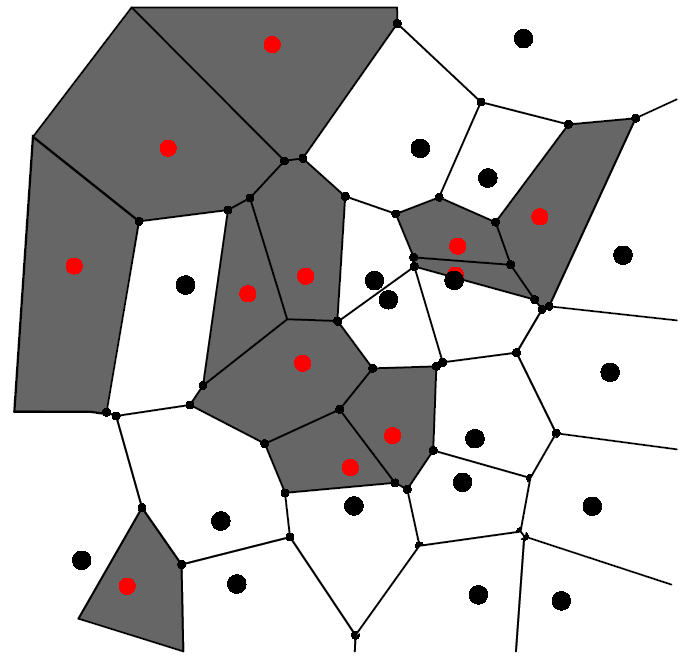
\includegraphics[width=8cm]{1627808452244-6.1-1.png}
  \caption{L2 范数 Voronoi 区域}
\end{figure}

证明:由余弦定理

\begin{equation}
a^{\top}b=\frac{\left\| a \right\|^2+\left\| b \right\|^2-\left\| a-b \right\|^2}{2}
\end{equation}

可知对 $\xi_1,\xi_2\in V_i$,

\begin{equation}
\xi =\lambda \xi_1+\left(1-\lambda \right)\xi_2,~\lambda \in \left[0,1 \right]
\end{equation}

有

\begin{equation}
\begin{aligned}
  \left\| \xi -x_i \right\|^2
  &=\lambda \left\| \xi_1-x_i \right\|^2-\lambda \left(1-\lambda \right)\left\| \xi_1-\xi_2 \right\|^2 +\left(1-\lambda \right)\left\| \xi_2-x_i \right\|^2\\
  &\leqslant \left\| \xi -x_j \right\|^2,~\forall~j\ne i
\end{aligned}
\end{equation}

平均错误率:

\begin{equation}
P_N\left(e \right)=\iint{P_N\left(e|x,x' \right)p\left(x'|x \right)\mathrm{d}x'p(x)\mathrm{d}x}
\end{equation}

渐进平均错误率:

\begin{equation}
P=\lim_{N\rightarrow \infty} P_N\left(e \right)
\end{equation}

记 Bayes 错误率为 $P^*$, 则渐进平均错误率的范围

\begin{equation}
P^*\leqslant P\leqslant P^*\left(2-\frac{c}{c-1}P^*\right)
\end{equation}

\begin{figure}
  \centering
  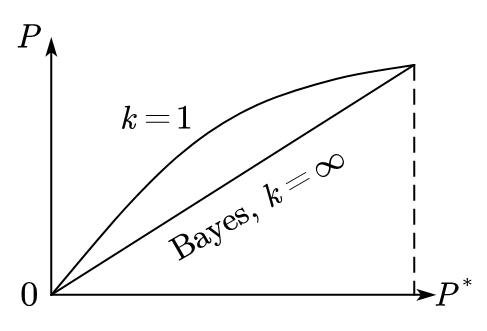
\includegraphics[width=8cm]{1627808484207-6.1-2.jpg}
  \caption{近邻法错误率与 Bayes 错误率对比}
\end{figure}

\section{\texorpdfstring{$k$}{k}-近邻法 (\texorpdfstring{$k$}{k} Nearest Neighbors)}

思想:测试样本与距离它最近的 $k$ 个样本中占优的类同类

算法:最近邻法寻找 $k$ 个近邻,$k_i$ 表示属于 $\omega_i$ 的样本数,判别函数 $g_i(x)=k_i$,决策规则

\begin{equation}
g_j(x)=\max_ik_i\Rightarrow x\in \omega_j
\end{equation}

\section{近邻法快速算法}

思想:样本集分级分解成多个子集 (树状结构) ,每个子集 (结点) 可用较少几个量代表,通过将新样本与各结点比较排除大量候选样本,只与最终结点 (子集) 中逐个样本比较

\section{压缩近邻法 (Condensing) }

算法:关注两类边界附近的样本,初始 Grabbag 为全部样本

1. 从 Grabbag 中选择一个样本放入 Store 中

2. 用 Store 中样本以近邻法测试 Grabbag 中样本,若分错则将该样本放入 Store

3. 重复 2) 直到 Grabbag 中没有样本再转到 Store 中,或 Grabbag 为空则停止

4. 用 Store 中样本作为近邻法设计集

\section{距离度量}

距离定义:二元函数 $D\left(\cdot ,\cdot \right)$

1. 自反性:$D\left(x,y \right)=0\Leftrightarrow x=y$

2. 对称性:$D\left(x,y \right)=D\left(y,x \right)$

3. 三角不等式:$D\left(x,y \right)+D\left(y,z \right)\geqslant D\left(x,z \right)$

注释:非负性 $D\left(x,y \right)\geqslant 0$ 可由定义三条性质导出

Minkowski 距离度量:

\begin{equation}
D\left(x,y \right)=\left(\sum_{j=1}^{d}|x_j-y_j|^s \right)^{1/s},~s\geqslant 1
\end{equation}

欧氏距离:

\begin{equation}
D\left(x,y \right)=\left\| x-y \right\|_2=\sqrt{\left(x-y \right)^{\top}\left(x-y \right)}
\end{equation}

Chebychev 距离:

\begin{equation}
D\left(x,y \right)=\left\| x-y \right\|_{\infty}=\max_j|x_j-y_j|
\end{equation}

马氏距离:可以表示样本距离对样本分布 (主要是方差) 的依赖性

\begin{equation}
D\left(x,y \right)=\left(x-y \right)^{\top}\Sigma ^{-1}\left(x-y \right),~\Sigma =AA^{\top}
\end{equation}

且变换后等价于欧氏距离平方:

\begin{equation}
A^{-1}:x\mapsto x'\Rightarrow D\left(x,y \right)=\left\| x'-y' \right\|_{2}^{2}
\end{equation}

概率分布相似性判据:基于类条件概率密度函数

1. Bhattacharyya 距离:
  \begin{equation}
  J_B=-\ln \int \left[p\left(x|\omega_1 \right)p\left(x|\omega_2 \right)\right] ^{1/2}\mathrm{d}x
  \end{equation}
2. Chernoff 界限:
  \begin{equation}
  J_C=-\ln \int p^s\left(x|\omega_1 \right)p^{1-s}\left(x|\omega_2 \right)\mathrm{d}x
  \end{equation}
3. 散度:
  \begin{equation}
  J_D=\int \left[p\left(x|\omega_1 \right)-p\left(x|\omega_2 \right)\right] \ln\frac{p\left(x|\omega_1 \right)}{p\left(x|\omega_2 \right)} \mathrm{d}x
  \end{equation}

散度定义来源:

\begin{equation}
D\left(f_1,f_2 \right)=\int f_1(x)\ln\frac{f_1(x)}{f_2(x)} \mathrm{d}x
\end{equation}

\begin{equation}
J_D=D\left(f_1,f_2 \right)+D\left(f_2,f_1 \right)
\end{equation}

切距离:记 $y$ 所处流形的切空间基矩阵为 $T$, 则切距离为

\begin{equation}
D\left(x,y \right)=\min_a\left\| \left(y+aT \right)-x \right\|
\end{equation}

Holder 不等式:

\begin{equation}
\sum_{k=1}^{n}a_kb_k\leqslant \left\| a \right\|_p\left\| b \right\|_q,~\frac{1}{p}+\frac{1}{q}=1
\end{equation}

Minkowski 不等式:

\begin{equation}
\left\| a+b \right\|_p\leqslant \left\| a \right\|_p+\left\| b \right\|_p,~p\geqslant 1
\end{equation}

\chapter{特征提取与选择}

模式识别系统构成:

1. 数据获取→特征提取与选择→分类器设计

2. 数据获取→特征提取与选择→测试

\section{Fisher 线性判别}

思想:把 $d$ 维空间的样本投影到分开得最好的一条直线上

样本:

\begin{equation}
X=\{ x_1,\dots,x_N\} =X_1+X_2
\end{equation}

其中

\begin{equation}
|X_1|=N_1,~|X_2|=N_2
\end{equation}

降维:$y_n=w^{\top}x_n$,寻找最好的投影方向即寻找 $w$

样本均值:

\begin{equation}
m_i=\frac{1}{N_i}\sum_{x\in X_i}x
\end{equation}

类内离散度矩阵:

\begin{equation}
S_i=\sum_{x\in X_i}\left(x-m_i \right)\left(x-m_i \right)^{\top}
\end{equation}

总类内 (within-class) 离散度:$S_w=\sum_iS_i$,一般可逆

类间 (between-class) 离散度:

\begin{equation}
S_b=\left(m_1-m_2 \right)\left(m_1-m_2 \right)^{\top}
\end{equation}

一维投影空间:样本均值

\begin{equation}
\tilde{m}_i=\frac{1}{N_i}\sum_{y\in Y_i}y
\end{equation}

类内离散度

\begin{equation}
\tilde{S}_{i}^{2}=\sum_{y\in Y_i}\left(y-\tilde{m}_i \right)^2
\end{equation}

总类内离散度

\begin{equation}
\tilde{S}_w=\tilde{S}_{1}^{2}+\tilde{S}_{2}^{2}
\end{equation}

Fisher 准则函数:

\begin{equation}
J_F\left(w \right)=\frac{\left(\tilde{m}_1-\tilde{m}_2 \right)^2}{\tilde{S}_{1}^{2}+\tilde{S}_{2}^{2}}
\end{equation}

优化问题:广义 Rayleigh 商

\begin{equation}
\max~J_F\left(w \right)=\frac{w^{\top}S_bw}{w^{\top}S_ww}
\end{equation}

令分母为非零常数 $w^{\top}S_ww=c\ne 0$,可定义 Lagrange 函数

\begin{equation}
L\left(w,\lambda \right)=w^{\top}S_bw-\lambda \left(w^{\top}S_ww-c \right)
\end{equation}

由梯度条件可得

\begin{equation}
S_bw^*=\lambda S_ww^*
\end{equation}

即

\begin{equation}
\begin{aligned}
  \lambda w^*
  &=S_{w}^{-1}S_bw^*\\
  &=S_{w}^{-1}\left(m_1-m_2 \right)R
\end{aligned}
\end{equation}

其中

\begin{equation}
R=\left(m_1-m_2 \right)^{\top}w
\end{equation}

忽略比例因子 $R/\lambda$ 有

\begin{equation}
w^*=S_{w}^{-1}\left(m_1-m_2 \right)
\end{equation}

一维分类:估计类条件概率密度函数,采用 Bayes 决策,或取决策边界

\begin{equation}
\begin{aligned}
  y_{0}^{\left(1 \right)}&=\frac{\tilde{m}_1+\tilde{m}_2}{2}\\
  y_{0}^{\left(2 \right)}&=\frac{N_2\tilde{m}_1+N_1\tilde{m}_2}{N}
\end{aligned}
\end{equation}

注释:Fisher 适合正态分布数据,若投影到平面则可把两类切割开组成多类,$S_w$ 不可逆则数据有冗余,降维到可逆

多类 Fisher 线性判别:$K$ 类则最多可选取 $K-1$ 个特征

\section{类别可分性判据}

基于类内类间距离:

\begin{equation}
\begin{aligned}
  J_2&=\mathrm{Tr}\left(S_{w}^{-1}S_b \right)\\
  J_3&=\ln\frac{|S_b|}{|S_w|}\\
  J_4&=\frac{\mathrm{Tr}\left(S_b \right)}{\mathrm{Tr}\left(S_w \right)}\\
  J_5&=\frac{|S_w+S_b|}{|S_w|}\\
\end{aligned}
\end{equation}

基于概率分布:$J_B,~J_C,~J_D$

基于熵函数:

\begin{equation}
J_{c}^{\alpha}=\left(2^{1-\alpha}-1 \right)^{-1}\left[\sum_{i=1}^{c}P^{\alpha}\left(\omega_i|x \right)-1 \right]
\end{equation}

其中参数 $\alpha \rightarrow 1$:Shannon 熵,$\alpha =2$:平方熵

\section{特征提取}

降维:$x\in \mathbb{R} ^D\mapsto y\in \mathbb{R} ^d$,

\begin{equation}
y=W^{\top}x,~W\in \mathbb{R} ^{D\times d}
\end{equation}

优化问题:$S_{w}^{-1}S_b$ 前 $d$ 个特征值对应的特征向量组成 $W$

\section{特征选择}

问题:单独最好的 $d$ 个特征组合起来不一定是最好的

最优搜索算法:穷举法,分枝定界法

次优搜索算法:单独最优特征组合

1. 单独最优特征组合:
\begin{equation}
  J(x)=\sum_iJ\left(x_i \right)~\mathrm{or}~ \prod_iJ\left(x_i \right)
\end{equation}

2. 顺序前进法:单独最好+合作最好+合作最好

3. 顺序后退法:全部-合作最不好-合作次不好

4. 增 $l$ 减 $r$ 法:增加合作最好的,删除合作最不好的

5. 智能算法:模拟退火,遗传算法,Tabu 搜索

Relief 算法:

输入:训练集 $X=\left\{ x_i\in \mathbb{R} ^d \right\}_{i=1}^{N}$ 

随机选择样本数 $n$

设定 $d$ 维权重向量 

\begin{equation}
w=[w_1,w_2,…,w_D]^{\top}=0
\end{equation}

for $i=1$ to $n$:

从 $X$ 中随机选择一个样本 $x$

计算 $X$ 中离 $x$ 最近的同类样本 $h$,不同类的样本 $m$

for $j=1$ to $d$:

\begin{equation}
w_j=w_j-\frac{\mathrm{diff}(j,x,h)}{n}+\frac{\mathrm{diff}(j,x,m)}{n}
\end{equation}

return $w$

输出:权重 $w$ 最大的前 $k$ 个特征

差异计算:$\mathrm{diff(}j,x,h)$ 表示 $x$ 与 $h$ 在第 $j$ 维上绝对值的差异

1. 离散变量:
  \begin{equation}
  \mathrm{diff}(j,x,h)=1-\left[x_j=h_j \right]
  \end{equation}
2. 连续变量:
  \begin{equation}
  \mathrm{diff}(j,x,h)=\frac{|x_j-h_j|}{x_{j\max}-x_{j\min}}
  \end{equation}

\chapter{深度学习}

\section{Multi-Layer Perception, MLP}

Perceptron:单个神经元→感知器

\begin{figure}
  \centering
  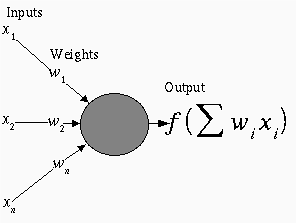
\includegraphics[width=8cm]{1627808551310-8.1.png}
  \caption{感知器[1]}
\end{figure}

$x=\left[x_1,\dots ,x_p \right] ^{\top}, w=\left[w_1,\dots ,w_p \right] ^{\top}$

神经元输入 $v=w^{\top}x-\theta$

\begin{equation}
  y=\mathrm{sgn}(v)=
  \begin{cases}
    +1, &\mathrm{if}~v\geqslant 0\\
    -1, &\mathrm{if}~v< 0\\
  \end{cases}
\end{equation}

激活函数:

1. 符号函数:
  \begin{equation}
  \phi(x)=\mathrm{sgn}(x)
  \end{equation}
2. Sigmoid:
  \begin{equation}
  \phi(x)=\frac{1}{1+\exp(-x)}
  \end{equation}
3. 分段线性函数
4. ReLU:
  \begin{equation}
  \phi (x)=
  \begin{cases}
    x, &\mathrm{if}~x\geqslant0\\
    0, &\mathrm{if}~x<0\\
  \end{cases}
  \end{equation}
5. Leaky ReLU:
  \begin{equation}
  \phi (x)=
  \begin{cases}
    x, &\mathrm{if}~x\geqslant 0\\
    ax, &\mathrm{if}~x<0\\
  \end{cases}
  \end{equation}
6. Softmax:
  \begin{equation}
  \phi(x)=\frac{\exp(x)}{1^{\top}\exp(x)}
  \end{equation}
7. 双曲正切:
  \begin{equation}
  \phi (x)=\tanh (x)=\frac{\mathrm{e}^x-\mathrm{e}^{-x}}{\mathrm{e}^x+\mathrm{e}^{-x}}
  \end{equation}

Multi-Layer Perceptron:多层感知机网络

逼近能力:$\forall f\in C^{\left[0,1 \right] ^p}, \epsilon >0, \exists~M,\alpha ,\theta ,w$

\begin{equation}
F(x)=\sum_{i=1}^{M}\alpha_i\phi \left(\sum_{j=1}^{p}w_{ij}x_j-\theta_i \right)
\end{equation}

使得

\begin{equation}
|F(x)-f(x)|<\epsilon
\end{equation}

标签:one-hot vector

\begin{equation}
y=\left[0,\dots ,0,1,0,\dots ,0 \right]
\end{equation}

交叉熵损失:$L=-y^{\top}\ln \hat{y}$,$\hat{y}$ 为网络输出判别结果

均方误差损失:样本集 $X=\left\{ x_n \right\}_{n=1}^{N}$,标签为 $\left\{ d\left(n \right)\right\}$

输出端第 $j$ 个单元对第 $n$ 个样本的输出:$y_j\left(n \right)$

第 $j$ 个单元的误差信号:

\begin{equation}
e_j\left(n \right)=d_j\left(n \right)-y_j\left(n \right)
\end{equation}

输出端对第 $n$ 个样本的平方误差:

\begin{equation}
E\left(n \right)=\frac{1}{2}\sum_{j=1}^{c}e_{j}^{2}\left(n \right)
\end{equation}

全部 $N$ 个样本的平方误差均值:

\begin{equation}
E_{\mathrm{av}}=\frac{1}{N}\sum_{n=1}^{N}E\left(n \right)
\end{equation}

逐个样本学习的 BP 算法:

1) 误差对输出单元 $j$ 的权重 $\left\{ w_{ji},~\forall~i \right\}$ 求梯度

由

\begin{equation}
v_j\left(n \right)=\sum_{i=0}^{p}w_{ji}\left(n \right)y_i\left(n \right)
\end{equation}

\begin{equation}
y_j\left(n \right)=\phi_j\left(v_j\left(n \right)\right)
\end{equation}

可得

\begin{equation}
\begin{aligned}
  \frac{\partial E\left(n \right)}{\partial w_{ji}\left(n \right)}
  &=\frac{\partial E\left(n \right)}{\partial e_j\left(n \right)}\frac{\partial e_j\left(n \right)}{\partial y_j\left(n \right)}\frac{\partial y_j\left(n \right)}{\partial v_j\left(n \right)}\frac{\partial v_j\left(n \right)}{\partial w_{ji}\left(n \right)}\\
  &=-e_j\left(n \right)\phi_{j}^{'}\left(v_j\left(n \right)\right)y_i\left(n \right)\\
  &:=\delta_j\left(n \right)y_i\left(n \right)
\end{aligned}
\end{equation}

权重修正:

\begin{equation}
w_{ji}=w_{ji}+\eta \delta_j\left(n \right)y_i\left(n \right)
\end{equation}

其中 $\delta_j\left(n \right)$ 称为局部梯度

2) 误差对内部隐单元 $j$ 的权重 $\left\{ w_{ji},~\forall~i \right\}$ 求梯度

局部梯度为

\begin{equation}
\begin{aligned}
  \delta_j\left(n \right)
  &=-\frac{\partial E\left(n \right)}{\partial y_j\left(n \right)}\frac{\partial y_j\left(n \right)}{\partial v_j\left(n \right)}\\
  &=-\frac{\partial E\left(n \right)}{\partial y_j\left(n \right)}\phi_{j}^{'}\left(v_j\left(n \right)\right)
\end{aligned}
\end{equation}

其中

\begin{equation}
\begin{aligned}
  \frac{\partial E\left(n \right)}{\partial y_j\left(n \right)}
  &=\sum_k{\frac{\partial E\left(n \right)}{\partial e_k\left(n \right)}\frac{\partial e_k\left(n \right)}{\partial y_k\left(n \right)}\frac{\partial y_k\left(n \right)}{\partial v_k\left(n \right)}\frac{\partial v_k\left(n \right)}{\partial y_j\left(n \right)}}\\
  &=-\sum_ke_k\phi '\left(v_k\left(n \right)\right)w_{kj}\left(n \right)\\
  &=-\sum_k\delta_k\left(n \right)w_{kj}\left(n \right)
\end{aligned}
\end{equation}

因此

\begin{equation}
\delta_j\left(n \right)=\phi_{j}^{'}\left(v_j\left(n \right)\right)\sum_k\delta_k\left(n \right)w_{kj}\left(n \right)
\end{equation}

权重修正:

\begin{equation}
w_{ji}=w_{ji}+\eta \delta_j\left(n \right)y_i\left(n \right)
\end{equation}

BP 问题:局部极值且收敛缓慢,需大量数据已知网络结构

深度问题:更深的深度可以具有更好的表示性但优化更困难

例题:$k$ 类,输入 $x\in \mathbb{R} ^d$,one-hot 标签 $y\in \mathbb{R} ^k$,交叉熵损失网络为

\begin{equation}
\begin{aligned}
  \hat{y}&=f\left(x;W_1,b_1,W_2,b_2 \right)\\ 
  h_1&=W_{1}^{\top}x+b_1 \\
  a_1&=\mathrm{ReLU}\left(h_1 \right)\\
  h_2&=\begin{bmatrix}
    a_1\\ x
  \end{bmatrix} \\
  a_2&=h_2\odot m \\
  h_3&=W_{2}^{\top}a_2+b_2 \\
  \hat{y}&=\mathrm{Softmax}\left(h_3 \right)
\end{aligned}
\end{equation}

则损失函数对各个变量的梯度为

\begin{equation}
\begin{aligned}
  \bar{\hat{y}}&=-y\hat{y} \\
  \bar{h}_3&=\hat{y}-y \\
  \bar{W}_2&=a_2\bar{h}_{3}^{\top} \\
  \bar{b}_2&=\bar{h}_3 \\
  \bar{a}_2&=W_2\bar{h}_3\\
  \bar{h}_2&=m\odot \bar{a}_2 \\
  \bar{a}_1&=\left[I~~0 \right] \bar{h}_2 \\
  \bar{h}_1&=\mathrm{diag}\left[\frac{1+\mathrm{sgn} \left(h_1 \right)}{2}\right]\bar{a}_1\\
  \bar{W}_1&=x\bar{h}_{1}^{\top} \\
  \bar{b}_1&=\bar{h}_1 \\
  \bar{x}&=W_1\bar{h}_1+\left[0~~I\right] \bar{h}_2
\end{aligned}
\end{equation}

\section{Convolutional Neural Networks (CNN)}

Dropout:随机删除某个节点的连接,以重点关注其余节点

例题:输入 $x\in \mathbb{R} ^{C_{\mathrm{in}}\times H\times W}$, 

\begin{equation}
\begin{aligned}
  u_1&=\mathrm{Conv}2\mathrm{d}\left(C_{\mathrm{in}},C_{\mathrm{out}},k \right)(x)\\
  h_1&=\mathrm{MaxPoil}2\mathrm{d}\left(N \right)\left(u_1 \right) \\
  a_1&=\mathrm{ReLU}\left(h_1 \right) \\
  u_2&=\mathrm{Flatten}\left(a_1 \right)\\
  h_2&=W_{2}^{\top}u_2+b_2 \\
  \hat{y}&=\mathrm{Softmax} \left(h_2 \right)\\
\end{aligned}
\end{equation}

则损失函数对各个变量的梯度为

\begin{equation}
\begin{aligned}
  \bar{h}_2&=\hat{y}-y \\
  \bar{W}_2&=a_2\bar{h}_{2}^{\top}\\
  \bar{b}_2&=\bar{h}_2 \\
  \bar{u}_2&=W_2\bar{h}_2 \\
  \bar{a}_{1}^{\left(i,j,k \right)}&=W_{2}^{\left(n\left(i,j,k \right),: \right)}\bar{h}_2
\end{aligned}
\end{equation}

其中 

\begin{equation}
n\left(i,j,k \right)=\left(i-1 \right)H_{\mathrm{mp}}W_{\mathrm{mp}}+\left(j-1 \right)W_{\mathrm{mp}}+k
\end{equation}

\begin{equation}
\bar{h}_{1}^{(r,s,t)}=\frac{1+\mathrm{sgn} \left(h_{1}^{(r,s,t)} \right)}{2} \bar{a}_{1}^{(r,s,t)}
\end{equation}

卷积:

\begin{equation}
u_{1}^{\left(j,:,: \right)}=b_{1}^{\left(j,:,: \right)}+\sum_{k=1}^{C_{\mathrm{in}}}W_{1}^{\left(j,k,:,: \right)}\star x^{\left(k,:,: \right)}
\end{equation}

其中 $\star$ 符号表示二维互相关

例题:

\begin{equation}
a_i=\mathrm{Sigmoid}\left(W_{i}^{\top}a_{i-1}+b_i \right),~i=1,\dots ,l
\end{equation}

且

\begin{equation}
a_0=x, a_l=\hat{y}
\end{equation}

令

\begin{equation}
\sigma \left(z \right):=\mathrm{Sigmoid}\left(z \right)
\end{equation}

则

\begin{equation}
\sigma '\left(z \right)=\mathrm{diag}\left(\sigma \left(z \right)\odot \left[1-\sigma \left(z \right)\right] \right)
\end{equation}

因此

\begin{equation}
\bar{W}_1=x\left[\left(\prod_{i=2}^{l}W_i \right)\left(\prod_{j=1}^{l}\sigma '\left(a_j \right)\right)\bar{\hat{y}} \right] ^{\top}
\end{equation}

其中

\begin{equation}
\sigma '\left(a_j \right)\leqslant \frac{1}{4}
\end{equation}

则会出现梯度消失的问题

ReLU:

\begin{equation}
\bar{W}_1=x\left[\left(\prod_{i=2}^{l}W_i \right)\left(\prod_{j=1}^{l}\mathrm{diag}\left[\frac{1+\mathrm{sgn} \left(a_j \right)}{2}\right] \right)\bar{\hat{y}} \right] ^{\top}
\end{equation}

若行列式 $\mathrm{det}(W_i)$ 过小,则其连乘部分会消失,整体的梯度仍然会消失

ResNet:

\begin{equation}
a_i=\mathrm{Sigmoid}\left(W_{i}^{\top}a_{i-1}+b_i \right)+a_{i-1},i=1,\dots ,l
\end{equation}

则梯度为

\begin{equation}
\bar{W}_1=x\left[\sigma '\left(a_1 \right)\left(\prod_{i=2}^{l}\left[ W_i\sigma '\left(a_i \right)+I \right] \right)\bar{\hat{y}} \right] ^{\top}
\end{equation}

连乘的每一项都包含单位矩阵 $I$,有效缓解了梯度消失的问题

\section{Recurrent Neural Networks (RNN)}

目的:处理序列数据,如语言,轨迹,金融数据等

网络结构及展开:

\begin{figure}
  \centering
  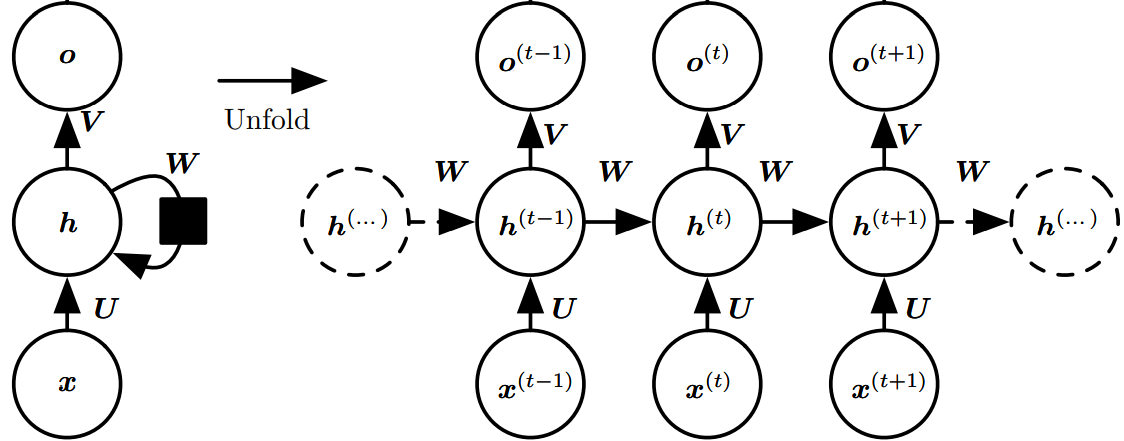
\includegraphics[width=10cm]{1627808597430-8.3.png}
  \caption{RNN 网络结构}
\end{figure}

更新方程:

\begin{equation}
\begin{aligned}
  h^{\left(t \right)}&=\phi \left(Wh^{\left(t-1 \right)}+Ux^{\left(t \right)}+b \right)\\ 
  \hat{y}^{\left(t \right)}&=\sigma \left(Vh^{\left(t \right)}+c \right)
\end{aligned}
\end{equation}

BP 算法:换个符号,并考虑 $E_t=d_t-y_t$

\begin{figure}
  \centering
  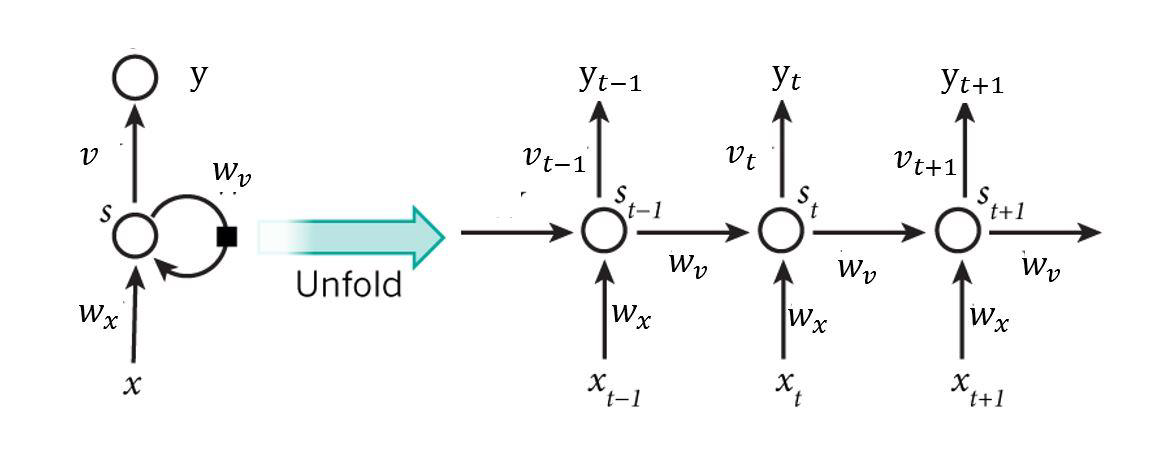
\includegraphics[width=10cm]{1627808617206-8.3-2.png}
  \caption{RNN 网络结构}
\end{figure}

$y_t=\phi \left(v_t \right), v_t=\sigma \left(w_vy_{t-1}+w_xx_t \right)$,这里 $\sigma (x):=x$

\begin{equation}
\begin{aligned}
  \frac{\partial E}{\partial w_v}&=\sum_{t=1}^s{\frac{\partial E_t}{\partial w_v}} \\
  \frac{\partial E_t}{\partial w_v}&=\sum_{k=1}^t{\frac{\partial E_t}{\partial y_t}\frac{\partial y_t}{\partial v_t}\frac{\partial v_t}{\partial v_k}\frac{\partial v_k}{\partial w_v}}\\
  \frac{\partial E_t}{\partial y_t}&=\frac{\partial \left(d_t-y_t \right)}{\partial y_t}=-1 \\
  \frac{\partial y_t}{\partial v_t}&=\phi '\left(v_t \right) \\
  \frac{\partial v_t}{\partial v_k}
  &=\prod_{i=k+1}^t{\frac{\partial v_i}{\partial v_{i-1}}}\\
  &=\prod_{i=k+1}^t{\frac{\partial v_i}{\partial y_{i-1}}\frac{\partial y_{i-1}}{\partial v_{i-1}}}\\
  &=\prod_{i=k+1}^t{w_v\phi '\left(v_{i-1} \right)}\\
  \frac{\partial v_k}{\partial w_v}&=y_{k-1}
\end{aligned}
\end{equation}

\section{Long Short Term Memory (LSTM)}

网络结构:对 RNN 的输入输出和展开过程均加入门控

\begin{figure}
  \centering
  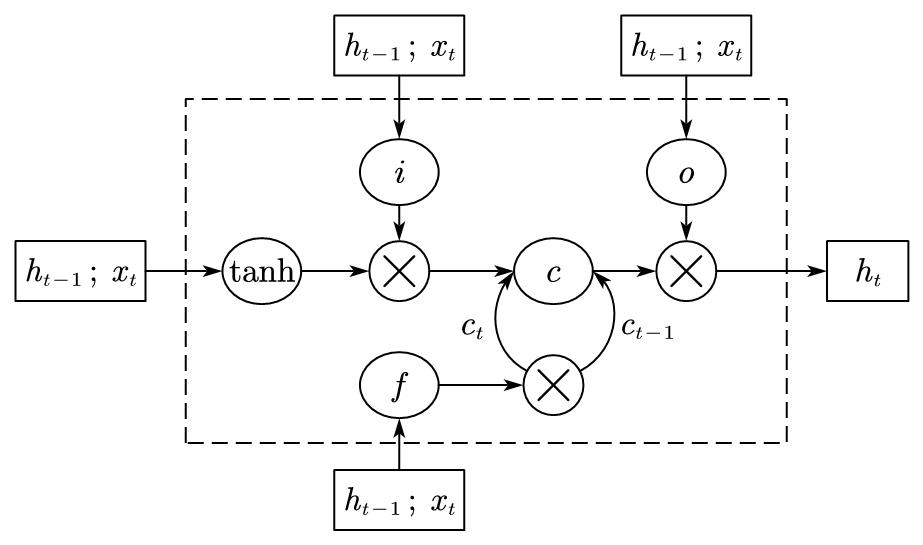
\includegraphics[width=10cm]{1627808642695-8.4.jpg}
  \caption{LSTM 网络结构}
\end{figure}

更新过程:$\sigma \left(\cdot \right):=\mathrm{sigmoid}\left(\cdot \right)$

Input gate:$i_t=\sigma \left(w_{xi}x_t+w_{hi}h_{t-1}+b_i \right)$

Forget gate:$f_t=\sigma \left(w_{xf}x_t+w_{hf}h_{t-1}+b_f \right)$

Output gate:$o_t=\sigma \left(w_{xo}x_t+w_{ho}h_{t-1}+b_o \right)$

External input gate:

\begin{equation}
g_t=\tanh \left(w_{xg}x_t+w_{hg}h_{t-1}+b_g \right)
\end{equation}

输出:

\begin{equation}
\begin{aligned}
  c_t&=f_t\odot c_{t-1}+i_t\odot g_t\\
  h_t&=o_t\odot \tanh \left(c_t \right)
\end{aligned}
\end{equation}

梯度:

\begin{equation}
\begin{aligned}
  \bar{c}_t&=\bar{h}_to_t\left[1-\tanh^2\left(c_t \right)\right] \\
  \bar{w}_{ix}&=\sum_t\bar{i}_ti_t\left(1-i_t \right)x_t
\end{aligned}
\end{equation}

\section{Attention}

注意力机制:加权平均,权重表示不同的重视程度

网络参数:键值对 $\left\{ k_i,v_i \right\}$,查询向量 $q$

注意力:

\begin{equation}
\begin{aligned}
  c\left(\left\{ k_i,v_i \right\} ,q \right)&=\sum_i\mathrm{similarity}\left(q,k_i \right)\cdot v_i\\
  &=\sum_i\alpha_iv_i
\end{aligned}
\end{equation}

相似性度量:$\alpha_i$ 的计算可使用内积,余弦相似度,MLP,softmax:

\begin{equation}
\alpha_i=\frac{\exp \left(k_{i}^{\top}q \right)}{\sum_i\exp \left(k_{i}^{\top}q \right)}
\end{equation}

\section{Graph Convolutional Neural Networks (GNN)}

邻接矩阵:$A=\left[a_{ij} \right],~a_{ij}=\left[i\rightarrow j \right]$

度矩阵:$D=\mathrm{diag}\left(d_i \right)$,出度 $d_i=\sum_ja_{ij}$,入度 $d_j=\sum_ia_{ij}$

简单 Propagation:

\begin{equation}
H^{i+1}=\sigma \left(D^{-1}AH^iW^i \right)
\end{equation}

\chapter{非监督学习:降维}

降维:给定一组高维样本,寻找一个低维空间表示这些样本

\section{主成分分析 (PCA, Principal Component Analysis) }

理论推导:最小均方误差的角度

向量 $x\in \mathbb{R} ^n$ 视为随机变量,完备正交归一向量基:$\left\{ u_i \right\}_{i=1}^{\infty}$,则 

\begin{equation}
x=\sum_{i=1}^{\infty}c_iu_i
\end{equation}

若用 $d\ll n$ 维来表示有 

\begin{equation}
\hat{x}=\sum_{i=1}^{d}c_iu_i
\end{equation}

误差为

\begin{equation}
\epsilon =\mathbb{E} \left[\left(x-\hat{x} \right)^{\top}\left(x-\hat{x} \right)\right] =\mathbb{E} \left[\sum_{i=d+1}^{\infty}c_{i}^{2} \right]
\end{equation}

又 $c_i=x^{\top}u_i$,则

\begin{equation}
\begin{aligned}
  \epsilon 
  &=\mathbb{E} \left[\sum_{i=d+1}^{\infty}u_{i}^{\top}xx^{\top}u_i \right] \\
  &=\sum_{i=d+1}^{\infty}u_{i}^{\top}\mathbb{E} \left[xx^{\top} \right] u_i\\
  &=\sum_{i=d+1}^{\infty}u_{i}^{\top}\Psi u_i\\
\end{aligned}
\end{equation}

其中

\begin{equation}
\Psi :=\mathbb{E} \left[xx^{\top} \right]
\end{equation}

零均值化:须保证 $\mathbb{E} \left[x \right] =0$,则 $\Psi$ 为协方差矩阵

优化问题:$\min \epsilon$,其 Lagrange 函数为

\begin{equation}
L=\sum_{i=d+1}^{\infty}u_{i}^{\top}\Psi u_i-\sum_{i=d+1}^{\infty}\lambda_i\left(u_{i}^{\top}u_i-1 \right)
\end{equation}

梯度条件:

\begin{equation}
\frac{\partial L}{\partial u_j}=2\left(\Psi u_j-\lambda_ju_j \right)=0
\end{equation}

即

\begin{equation}
\Psi u_j=\lambda_ju_j
\end{equation}

K-L 变换坐标系:$\Psi$ 前 $d$ 个最大特征值对应的特征向量

K-L 变换:$x$ 在 $u_1,u_2,\dots ,u_d$ 上展开系数

\begin{equation}
x'=\left[c_1,c_2,\dots ,c_d \right] ^{\top}
\end{equation}

性质:视展开系数 $x'$ 为随机向量,

\begin{equation}
\mathbb{E} \left[c_ic_j \right] =\lambda_iu_{i}^{\top}u_j=\lambda_i\delta_{ij}
\end{equation}

\begin{equation}
\lambda_i=\mathbb{E} \left[c_{i}^{2} \right] =\mathbb{E} \left[\left(c_i-\mathbb{E} \left(c_i \right)\right)^2 \right] =\sigma_{i}^{2}
\end{equation}

即特征值 $\lambda_i$ 表示数据降维投影在一维特征向量 $u_i$ 方向上的方差,所以 K-L 变换就是把数据投影到 $d$ 个正交的序贯最大方差方向上去

降维维度确定:根据精度要求与计算、存储能力确定

\section{多维尺度变换 (MDS, Multi-Dimensional Scaling) }

理论推导:数据点 $x_r\in \mathbb{R} ^p, r=1,2,\dots ,n$,假定零均值

内积 $b_{rs}=x_{r}^{\top}x_s$,$X=\left[x_1,\dots ,x_n \right] ^{\top}$,内积矩阵为 $B=XX^{\top}$,平方距离

\begin{equation}
\begin{aligned}
  d_{rs}^{2}
  &=\left(x_r-x_s \right)^{\top}\left(x_r-x_s \right)\\
  &=x_{r}^{\top}x_r+x_{s}^{\top}x_s-2x_{r}^{\top}x_s
\end{aligned}
\end{equation}

平方距离矩阵

\begin{equation}
D=c1^{\top}+1c^{\top}-2B
\end{equation}

其中

\begin{equation}
c=\left[x_{1}^{\top}x_1,\dots ,x_{n}^{\top}x_n \right]
\end{equation}

中心化矩阵:

\begin{equation}
J=I-\frac{1}{n}11^{\top}
\end{equation}

易知

\begin{equation}
\left(c1^{\top} \right)J=J\left(1c^{\top} \right)=0
\end{equation}

且由 $\sum_rx_r=0$ 可得

\begin{equation}
JX=X-\frac{1}{n}11^{\top}X=X
\end{equation}

因此

\begin{equation}
JBJ=JXX^{\top}J^{\top}=B
\end{equation}

又

\begin{equation}
\begin{aligned}
  JDJ&=J\left(c1^{\top} \right)J+J\left(1c^{\top} \right)J-2JBJ\\
  &=-2B \\
\end{aligned}
\end{equation}

所以

\begin{equation}
B=-\frac{1}{2}JDJ
\end{equation}

SVD:$B=V\Lambda V^{\top}$,其中 $V=\left[v_1,\dots ,v_p \right]$,$\Lambda =\mathrm{diag}\left(\lambda_1,\dots ,\lambda_p \right)$,则 $X=V\Lambda ^{1/2}$,若降维 $k < p$ 则取前 $k$ 个特征值与特征向量

降维维度确定:

\begin{equation}
\begin{aligned}
  \frac{1}{2}\sum_r\sum_sd_{rs}^{2}
  &=n\sum_rx_{r}^{\top}x_r\\
  &=n\mathrm{Tr}\left(B \right)\\
  &=n\sum_r\lambda_r\\
\end{aligned}
\end{equation}

可知为保持总体距离降低较少需取较大的特征值,总体距离降低比例为 

\begin{equation}
\rho=\frac{\displaystyle\sum_{i=1}^{p}\lambda_i}{\displaystyle\sum_{i=1}^{n-1}\lambda_i}
\end{equation}

可通过固定比例为 $\rho=95\%$ 选取 $p$

\section{等距特征映射 (ISOMAP, Isometric Feature Mapping) }

基本思想:利用测地距离代替欧氏距离,保留样本分布信息

算法:

1. 找到 $k$ 近邻 (或欧氏距离小于 $\epsilon$) 点并计算欧式距离 $d_X\left(i,j \right)$,定义图 $G$,若样本点为 $k$ 近邻则连线,连线长度为 $d_X\left(i,j \right)$

2. 计算图上任意两点间最短距离 $D_G=\left[d_G\left(i,j \right)\right]$

3. 通过 MDS 多维尺度变换降维到 $d$ 维空间

\section{局部线性嵌入 (LLE, Locally Linear Embedding) }

基本思想:高维数据集中分布在潜在的低维的平滑流形上,每个样本点及其近邻分布在流形上的一个局部线性区域

1. 寻找每个样本点的近邻

2. 解优化问题
   \begin{equation}
   \min \epsilon \left(W \right)=\sum_i\left|x_i-\sum_jW_{ij}x_j\right|^2
   \end{equation} 
   求得 $W$

3. 固定 $W$,求降维向量
  \begin{equation}
  y_i\Leftarrow \min \epsilon \left(W \right)=\sum_i\left|x_i-\sum_jW_{ij}x_j\right|^2
  \end{equation}

\chapter{非监督学习:聚类}

\section{\texorpdfstring{$C$}{C} 均值方法 (K-means)}

基于样本的方法:根据样本间相似性,使准则函数 $J_e$ 取最值

思路:

1. 把样本分成一些不同的类别

2. 不断调整样本使得相似的样本聚集在一起

3. GMM 的 EM 算法取极限的特例

算法:

\begin{equation}
\min J_e=\sum_{i=1}^c{\sum_{y\in \Gamma_i}^{}{\left\| y-m_i \right\|^2}}
\end{equation}

1. 把样本初始划分成 $C$ 类,计算各类均值 $m_1,\dots ,m_C$ 和 $J_e$

2. 选任意一个样本 $y$,设 $y\in \Gamma_i$

3. 若 $N_i=1$,则该类只有1个元素则无需移出,转 2)

4. 计算当 $y$ 被调整到其它各类时 $J_e$ 的变化量:

\begin{equation}
  \rho_j=
  \begin{cases}
    \dfrac{N_j}{N_j+1}\left\| y-m_j \right\|^2, &\mathrm{if}~j\ne i\\
    \dfrac{N_i}{N_i-1}\left\| y-m_j \right\|^2, &\mathrm{o}.\mathrm{w}.
  \end{cases}
\end{equation}

5. 如果 $\rho_k\leqslant \rho_j, \forall j$,则移动 $y:\Gamma_i\rightarrow \Gamma_k$
6. 更新均值 $m_i, m_k$ 和均方误差 $J_e$
7. 若连续迭代 $N$ 次不变则算法终止,否则转 2)

问题:

+ $C$ 的确定:$J_e-C$ 曲线肘点

+ 初始划分:先选择一些代表点作为聚类的核心,然后把其余的点按某种方法分到各类中去,初始划分不当可能会使得问题陷入局部最优解

\section{多级聚类方法 (Hierarchical Clustering) }

算法:

1. 每个样本为一类

2. 最近的两类合并,直到只剩一类

两类之间的距离度量:

+ 最近距离:

  \begin{equation}
  \Delta \left(\Gamma_i,\Gamma_j \right)=\min_{y\in \Gamma_i, \tilde{y}\in \Gamma_j}\delta \left(y,\tilde{y} \right)
  \end{equation}

  不适合两类之间距离较近且中间有个别离群点,适合带状分布的数据

+ 最远距离:

  \begin{equation}
  \Delta \left(\Gamma_i,\Gamma_j \right)=\max_{y\in \Gamma_i, \tilde{y}\in \Gamma_j}\delta \left(y,\tilde{y} \right)
  \end{equation}

  与最近距离效果相反

+ 均值距离:

  \begin{equation}
  \Delta \left(\Gamma_i,\Gamma_j \right)=\delta \left(m_i,m_j \right)
  \end{equation}

  效果介于以上两者之间

分类数量:根据聚类树判断,最长或次长跳跃前的水平

\begin{figure}
  \centering
  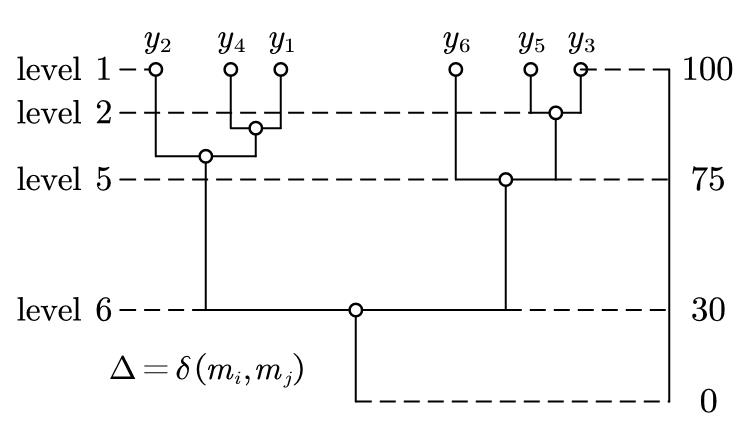
\includegraphics[width=8cm]{1627808686180-10.2.jpg}
  \caption{分级聚类示例}
\end{figure}

\section{谱聚类 (Spectral Clustering) }

样本点集:$x_1,\dots ,x_n$

相似性度量:$s_{ij}=s\left(x_i,x_j \right)\geqslant 0$

相似性图:加权无向图 $G=\left(V,E \right)$

加权邻接矩阵:$W=\left(w_{ij} \right)$

边权重:$w_{ij}=s_{ij}$

度矩阵:$D=\mathrm{diag}\left(d_1,\dots ,d_n \right)$,其中度:

\begin{equation}
d_i=\sum_{j=1}^{n}w_{ij}
\end{equation}

Graph Laplacian:未归一化 $L=D-W$,归一化 $L_{rw}=D^{-1}L$

性质:对称,半正定,最小特征值0,对应特征向量为1

构造相似性图:

1. $\epsilon$-近邻图:任意两个距离小于 $\epsilon$ 的点之间存在一条边

2. $k$-近邻图:若 $v_i$ 是 $v_j$ 的 $k$ 近邻,则存在一条边 (无向化) 

3. 对称 $k$-近邻图:若两个点互为 $k$ 近邻,则存在一条边

4. 全连接图:相似性大于 0 的两个点之间存在一条边

算法:

1. 输入相似性矩阵 $S\in \mathbb{R} ^{n\times n}$,聚类类别数 $k$

2. 构造相似性图,设加权邻接矩阵为 
\begin{equation}
  W=[w_{ij}]=[s_{ij}]
\end{equation}

3. 计算未归一化 (归一化) Graph Laplacian $L\left(L_{rw} \right)$

4. 计算 $L\left(Lu=\lambda Du \right)$ 的前 $k$ 个最小特征值对应的特征向量 $u_1,\dots ,u_k$,并记 
\begin{equation}
  U:=\left[u_1,\dots ,u_k \right]
\end{equation}

5. 设 $y_i\in \mathbb{R} ^k$ 为 $U$ 的第 $i$ 行构成的向量,称为谱嵌入向量

6. 使用 $C$ 均值聚类方法将点 $\left\{ y_i \right\}$ 聚为 $k$ 类 
  \begin{equation}
C_1,\dots ,C_k
\end{equation}

7. 输出最终聚类为 $A_1,\dots ,A_k$,其中 
\begin{equation}
  A_i=\left\{ j:y_j\in C_i \right\}
\end{equation}

推导:寻找图的划分,使得不同点集间边权重较小,同一点集内边权重较大,

\begin{equation}
\min \mathrm{cut}\left(A_1,\dots ,A_k \right)
=\frac{1}{2}\sum_{i=1}^{k}W\left(A_i,\bar{A}_i \right)
\end{equation}

其中 $|A|$ 表示 $A$ 中顶点的个数,$\mathrm{vol}\left(A \right)$ 表示 $A$ 中顶点度的和

\begin{equation}
\begin{aligned}
  \mathrm{RatioCut}\left(A_1,\dots ,A_k \right)
  &=\frac{1}{2}\sum_{i=1}^k{\frac{W\left(A_i,\bar{A}_i \right)}{|A_i|}}\\
  &=\frac{1}{2}\sum_{i=1}^k{\frac{\mathrm{cut}\left(A_i,\bar{A}_i \right)}{|A_i|}}
\end{aligned}
\end{equation}

\begin{equation}
\begin{aligned}
  \mathrm{NCut}\left(A_1,\dots ,A_k \right)
  &=\frac{1}{2}\sum_{i=1}^k{\frac{W\left(A_i,\bar{A}_i \right)}{\mathrm{vol}\left(A_i \right)}}\\
  &=\frac{1}{2}\sum_{i=1}^k{\frac{\mathrm{cut}\left(A_i,\bar{A}_i \right)}{\mathrm{vol}\left(A_i \right)}}
\end{aligned}
\end{equation}

松弛离散约束后,RatioCut 对应归一化 Graph Laplacian,Ncut 对应未归一化 Graph Laplacian

注记:

+ 谱聚类往往对相似性图及参数选择比较敏感,且存在尺度问题,一般 $k$ 近邻图可以比较好的连接不同尺度下的数据,通常作为首选

+ 参数选择应该使相似性图是连通的或连通分量数量较少

+ 尽量选择归一化的 Graph Laplacian,理由:考虑聚类的原则,最小化 RatioCut 只考虑了使得不同点集间的边的权重较小,而最小化 Ncut 在某种程度上考虑了同一点集内的边权重较大

聚类方法的选择:

+ 根据样本的分布特性和数量综合考虑

+ 若样本点近似成球状分布或者样本数很大时,则用 K-means 算法能取得较好效果,且速度快

+ 当样本数量较少时,可以选择基于最近邻图的谱聚类方法,其聚类的效果较好,而且不像分级聚类那样受距离度量选择的影响大

\chapter{决策树}

\section{决策树概览}

\begin{figure}
  \centering
  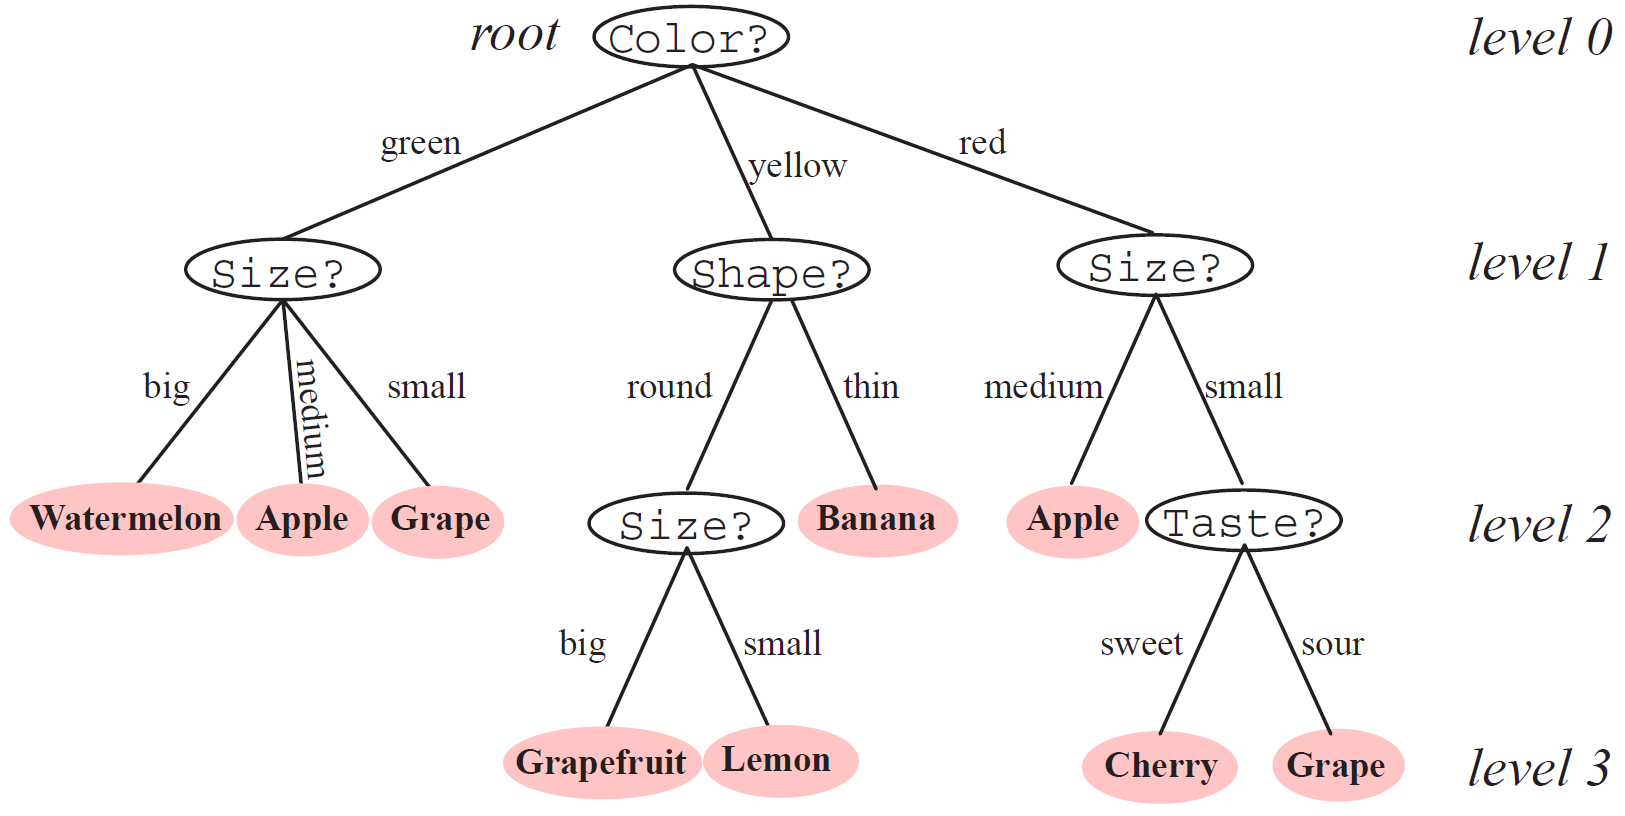
\includegraphics[width=8cm]{1627808711971-11.1.png}
  \caption{决策树示例}
\end{figure}

\section{CART (Classification And Repression Trees)}

分类和回归树算法 CART:一种通用的树生长算法

分枝数目:与属性有关,但决策树都等价于二叉树

构造决策树原则:简单性,获得的决策树简单、紧凑

节点不纯度 Impurity:$i\left(N \right)$ 表示节点 $N$ 的不纯度

+ 熵不纯度:
  \begin{equation}
  i\left(N \right)=-\sum_jP\left(w_j \right)\log_2P\left(w_j \right)
  \end{equation}
  其中 $P\left(w_j \right)$ 表示节点 $N$ 处属于 $w_j$ 类样本占节点总样本数的比例

+ Gini 不纯度:
  \begin{equation}
  \begin{aligned}
    i\left(N \right)
    &=\sum_{i\ne j}P\left(w_i \right)P\left(w_j \right)\\
    &=1-\sum_jP^2\left(w_j \right)
  \end{aligned}
  \end{equation}

+ 错分不纯度:被错分的最小概率 
  \begin{equation}
  i\left(N \right)=1-\max_jP\left(w_j \right)
  \end{equation}

\begin{figure}
  \centering
  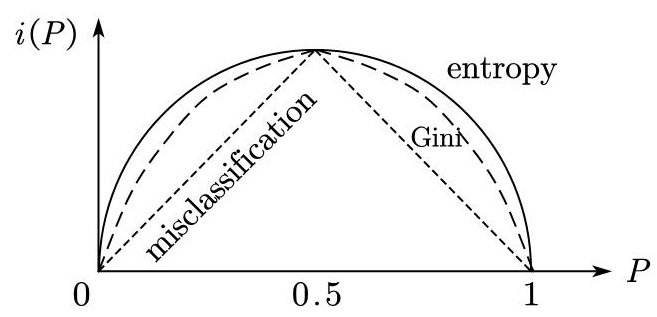
\includegraphics[width=8cm]{1627808735615-11.2.jpg}
  \caption{不纯度度量对比}
\end{figure}

特征选择:选择能够使不纯度下降最多的特征做查询,不纯度下降

\begin{equation}
\Delta i\left(N \right)=i\left(N \right)-P_Li\left(N_L \right)-\left(1-P_L \right)i\left(N_R \right)
\end{equation}

其中 $P_L$ 是分配到 $N_L$ 节点样本数量占 $N$ 节点样本数量比例

局部贪婪算法:只考虑了单一特征带来的不纯度下降

多重分枝:

\begin{equation}
\Delta i\left(N \right)=i\left(N \right)-\sum_{k=1}^{B}P_ki\left(N_k \right)
\end{equation}

其中 $B$ 为分枝数目,$P_k$ 是节点 $N_k$ 处样本占 $N$ 处样本比例,但

\begin{equation}
B\uparrow \Rightarrow \Delta i\left(N \right)\uparrow
\end{equation}

故调整

\begin{equation}
\Delta i_B\left(N \right)=
\frac{\Delta i\left(N \right)}{-\displaystyle\sum_{k=1}^{B}P_k\log_2P_k}
\end{equation}

分枝停止准则:

+ 传统方法,验证或交叉验证

+ 阈值方法,当所有候选分支的不纯度下降量都小于这个阈值,则停止分支

阈值方法优点:

+ 全部样本都可用来训练

+ 树的各个深度上都可能存在叶节点,这是一棵非平衡树

阈值方法缺点:
+ 很难预先设定一个合适的阈值,因为树的分类准确性与阈值大小通常不是简单的函数关系

后剪枝:使用全部训练集数据,但计算量会增加

1. 树充分生长,直到叶节点都有最小的不纯度值

2. 对所有相邻的成对叶节点,如果消去它们能引起不纯度增长,则消去它们,并令其公共父节点成为新的叶节点

叶节点标号:用叶节点样本中大多数样本的类别来标号

不稳定性:树的生长对训练样本的微小位置变动很敏感,很大程度上是由离散性和节点选择时的贪婪性所导致的

\begin{figure}
  \centering
  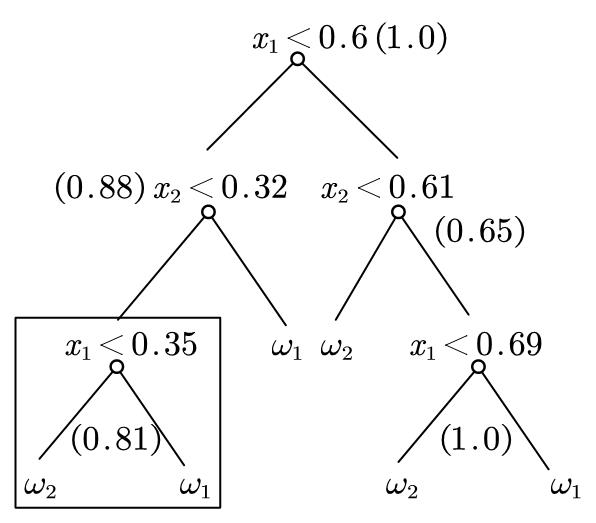
\includegraphics[width=8cm]{1627808769097-11.2(1).jpg}
  \caption{决策树构建与剪枝示例}
\end{figure}

特征选择:选择特征使得决策面简单,可尝试线性组合

多元决策树:当实值数据样本分布复杂时,平行于特征轴分界面的效率和推广性都可能很差,可采用一般的线性分类器

属性缺失:对主分支外的属性做替代分枝并根据相似性排序

\section{ID3 (Interactive Dichotomizer-3)}

算法:实值变量按区间离散化,节点分支数等于其属性的离散取值个数,决策树生长到所有叶节点都为纯,无剪枝

\section{C4.5}

算法概述:对于实值变量的处理和 CART 相同,对名义属性采用多重分支,不纯度的计算采用 $\Delta i_B\left(N \right)$

与 CART 区别:对属性缺失数据的处理,所有 $B$ 个分支进行判别,最终分类结果是 $M$ 个叶节点加权决策的结果

基于规则的剪枝:尝试删除规则任意一个前件,取性能提高最大的子规则,重复删除直到无法修剪,按性能降序排序

优点:

+ 允许在特定节点处考虑上下文信息

+ 靠近根节点处的节点也可能被剪枝,根节点与叶节点等价,比叶节点合并剪枝方法更加通用

+ 简化的规则可用于更好的类别表达

\chapter{多分类器方法 (Ensemble) }

\section{Bagging (Bootstrap Aggregating)}

算法:基于训练样本的分类器构造

1. 从训练集 $N$ 个样本中随机抽取 (Bootstrap) 出 $n$ 个样本

2. 用这 $n$ 个样本训练一个分类器 $h$,然后放回这些样本

3. 重复步骤 1) 与 2) $L$ 次,得到分类器 
\begin{equation}
  h_1, h_2,\dots ,h_L
\end{equation}

4. 使用 $L$ 个分类器进行判别,决策层投票得到最终结果

基分类器:选择不稳定的分类器,决策树,神经网络等

\section{AdaBoost (Adaptive Boosting)}

算法:基于训练样本的分类器构造

输入:$X=\left\{ \left(x_1,y_1 \right),\dots ,\left(x_N,y_N \right)\right\}$,基分类器 $C$,循环次数 $L$

初始化:样本 $x_i$ 权重

\begin{equation}
w_1(i)=\frac{1}{N}
\end{equation}

for $l=1$ to $L$:

权重归一化

\begin{equation}
p_l(i)=\frac{w_l(i)}{\displaystyle\sum_iw_l(i)},~\forall~i=1,2,\dots ,N
\end{equation}

根据 $p_l(i)$ 采样生成样本集合 $s_l$,训练分类器 $h_l$

计算 $h_l$ 分类错误率

\begin{equation}
\epsilon_l=\sum_ip_l(i)\bar{\delta}_{iy}
\end{equation}

其中

\begin{equation}
\bar{\delta}_{iy}:=\left[h_l\left(x_i \right)\ne y_i \right]
\end{equation}

计算权重系数的参数

\begin{equation}
a_l=\frac{1}{2}\ln\frac{1-\epsilon_l}{\epsilon_l}
\end{equation}

更新权重

\begin{equation}
w_{l+1}(i)=w_l(i)\mathrm{e}^{-a_l}\delta_{iy}+w_l(i)\mathrm{e}^{a_l}(1-\delta_{iy})
\end{equation}

输出:加权投票

\begin{equation}
h(x)=\mathrm{argmax}_{y\in Y}\sum_{l=1}^{L}a_l[h_l(x)=y]
\end{equation}

特性:随着算法进行,聚焦于容易分错而富含信息的样本

错误率:二分类 $Y=\left\{ 1,-1 \right\}$,$T$ 轮迭代后样本概率分布为

\begin{equation}
\begin{aligned}
  p_{T+1}(i)
  &=p_T(i)\frac{\mathrm{e}^{-\alpha_Ty_ih_T(i)}}{Z_T}\\
  &=p_1(i)\frac{\mathrm{e}^{-y_i\left< \alpha ,h(i)\right>}}{\displaystyle\prod_{j=1}^{T}Z_j}\\
  &=\frac{\mathrm{e}^{-y_i\left< \alpha ,h(i)\right>}}{N\displaystyle\prod_{j=1}^{T}Z_j}
\end{aligned}
\end{equation}

又

\begin{equation}
\sum_ip_{T+1}(i)=1 
\end{equation}

则

\begin{equation}
\prod_{j=1}^{T}Z_j=\frac{1}{N}\sum_{i=1}^N\mathrm{e}^{-y_i\left< \alpha ,h(i)\right>}
\end{equation}

第 $i$ 个样本错误标志

\begin{equation}
\begin{aligned}
  \epsilon_i
  &=1-\left[h_T\left(x_i \right)=y_i \right] \\
  &\leqslant \mathrm{e}^{-y_i\left< \alpha ,h(i)\right>}
\end{aligned}
\end{equation}

则总错误率是分类错误率的一个上界

\begin{equation}
\begin{aligned}
  \epsilon 
  &=\frac{1}{N}\sum_{i=1}^N\epsilon_i\\
  &\leqslant\frac{1}{N}\sum_{i=1}^N\mathrm{e}^{-y_i\left< \alpha ,h(i)\right>}\\
  &=\prod_{j=1}^{T}Z_j
\end{aligned}
\end{equation}

优化问题

\begin{equation}
\min~\prod_{j=1}^{T}Z_j
\end{equation}

可解得

\begin{equation}
a_l=\frac{1}{2}\ln\frac{1-\epsilon_l}{\epsilon_l}
\end{equation}

且由

\begin{equation}
\begin{aligned}
  Z_l
  &=\sum_ip_l(i)\mathrm{e}^{-\alpha_ly_ih_l(i)}\\
  &=\sum_{i\in A}p_l(i)\mathrm{e}^{-\alpha_l}+\sum_{i\in \bar{A}}p_l(i)\mathrm{e}^{+\alpha_l}\\
  &=\left(1-\epsilon_l \right)\mathrm{e}^{-\alpha_l}+\epsilon_l\mathrm{e}^{\alpha_l}\\
  &=2\sqrt{\epsilon_l\left(1-\epsilon_l \right)}\\
  &=\sqrt{1-4\gamma_{l}^{2}}
\end{aligned}
\end{equation}

可得

\begin{equation}
\begin{aligned}
  \prod_{l=1}^{T}Z_l
  &=\prod_{l=1}^{T}\sqrt{1-4\gamma_{l}^{2}}\\
  &\leqslant \exp \left(-2\sum_{l=1}^{T}\gamma_{l}^{2} \right)\\
  &\leqslant \mathrm{e}^{-2T\gamma_{\min}^{2}}
\end{aligned}
\end{equation}

因此,错误率可以随着迭代次数的增加而指数级下降

与 Bagging 对比:基分类器以序贯方式使用加权数据集进行训练,其中每个数据点权重依赖前一个分类器的性能

\section{基于样本特征的分类器构造}

随机子空间算法:随机抽取 (也可对特征加权) 特征子集 $S_l$,利用在 $S_l$ 上的训练样本训练分类器 $h_l$,重复 $L$ 次得到 $L$ 个分类器,最后进行投票

\begin{equation}
h(x)=\mathrm{argmin}_{y\in Y}\sum_{l=1}^{L}\left[h_l(x)=y \right]
\end{equation}

\section{分类器输出融合}

1. 决策层输出:对于待测试的样本,用每一个基分类器的分类结果投票,得票最多的类别号就是待测试样本的类别

2. 排序层输出:分类器输出为输入样本可能属于的类别列表,并依据可能性大小进行排序,之后采用 Borda 计数:对名次赋分,计算每个类别总得分并排序

3. 度量层输出:分类器输出为样本归属于各个类别的一种相似性度量,对于每一类的所有的相似性度量值求和,和值最大的类别就是未知样本的类别标号

\section{多分类器方法有效的原因}

1. 统计方面:避免单分类器分类时的不稳定性

2. 计算方面:脱离单分类器陷入的局部最优解

3. 表示方面:拓展原简单假设空间的表达能力

\chapter{统计学习理论}

\section{PAC (Probably Approximately Correct) 可学习}

若函数集 VC 维是有限值,则任意概率分布均 PAC 可学习

\section{VC (Vapnic-Chervonenkis) 维}

期望风险:

\begin{equation}
R\left(\omega \right)=\int L\left(y,f\left(x,\omega \right)\right)\mathrm{d}F\left(x,y \right)
\end{equation}

经验风险:

\begin{equation}
R_{\mathrm{emp}}\left(\omega \right)=\frac{1}{N}\sum_{i=1}^{N}L\left(y,f\left(x,\omega \right)\right)
\end{equation}

VC 维:描述学习机器的复杂性

推广性界定理:

\begin{equation}
R\left(\omega \right)\leqslant R_{\mathrm{emp}}\left(\omega \right)+\Phi \left(\frac{n}{\mathrm{VC}}\right)
\end{equation}

其中函数 $\Phi \searrow$

\section{没有免费的午餐}

+ 不存在一种模式分类算法具有天然的优越性,甚至不比随机猜测更好

+ 如果某种算法对某个特定的问题看上去比另一种算法更好,其原因仅仅是它更适合这一特定的模式分类任务

\section{丑小鸭定理}

不存在与问题无关的最好的特征集合或属性集合

\chapter{算法优缺点}

\section{贝叶斯分类器}

优点:

+ 理论上可以满足分类错误率最小

+ 对于服从特定模型的样本有较好的分类结果

+ 是其他分类算法的理论基础

缺点:

+ 依赖模型 (类先验概率,类条件概率分布的形式和具体参数) ,因此模型可能选错

+ 模型的参数可能过拟合

+ 实际样本独立同分布难以满足

\section{SVM}

优点:

+ 将低位空间线性不可分问题变换到高维空间,使其线性可分,由于只需要进内积计算,并没有增加多少计算复杂度

+ 推广能力与变换空间维数无关,具有较好的推广能力

+ 相对于传统方法,对模型具有一定的不敏感性

缺点:

+ 对大规模训练样本难以实施

+ 解决多分类问题存在困难

+ 对缺失数据敏感,对参数和核函数的选择敏感

\section{近邻法}

优点:

+ 错误率在贝叶斯错误率及其两倍之间

+ 算法直观容易理解易于实现

+ 可以适用任何分布的样本,算法适用性强

缺点:

+ 需将所有样本存入计算机中,每次决策都要计算待识别样本与全部训练样本的距离并进行比较,存储和计算开销大

+ 当错误的代价很大时,会产生较大风险

+ 错误率的分析是渐进的,这要求样本为无穷,实际中这一条件很难达到

\chapter{矩阵求导}

\section{迹 Trace}

\begin{equation}
\frac{\partial \mathrm{Tr}\left(W^{\top}\Sigma W \right)}{\partial W}=2\Sigma W
\end{equation}

\begin{equation}
\frac{\partial \mathrm{Tr}\left(AB \right)}{\partial A}=B+B^{\top}-\mathrm{diag}\left(B \right)
\end{equation}

\section{行列式}

\begin{equation}
\frac{\partial \ln |A|}{\partial A}=2A^{-1}-\mathrm{diag}\left(A^{-1} \right)
\end{equation}

\chapter{补充内容}

感知准则函数:
  \begin{equation}
  \min J_p\left(a \right)=\sum_{y\in Y^k}\left(-a^{\top}y \right)\geqslant 0
  \end{equation}
  以使错分样本到分界面距离之和最小为原则

分类器错误率:分类结果中与样本实际类别不同的样本在总体中的比例

错误率估计方法:理论计算,计算错误率的上界,实验估计

Fisher 与 Perceptron:Fisher 线性判别是把线性分类器的设计分为两步,一是确定最优方向,二是在这个方向上确定分类阈值;感知机则是通过不断迭代直接得到线性判别函数

K-means 与 EM (GMM):K 均值算法对数据点的聚类进行了硬分配,即每个数据点只属于唯一的聚类,而 EM 算法基于后验概率分布,进行了一个软分配。实际上,可以把 K 均值算法看成 GMM 的 EM 算法的一个特殊的极限情况。考虑高斯混合模型协方差矩阵均为 $\epsilon I$,从而

\begin{equation}
  P\left(x|\mu_k,\Sigma_k \right)=\frac{1}{\left(2\pi \epsilon \right)^{d/2}}\exp \left(-\frac{\left\| x-\mu_k \right\|^2}{2\epsilon}\right)
\end{equation}

令 $\epsilon \rightarrow 0$ 则可得到 K 均值算法的硬分配

\backmatter
\chapter{参考文献}

[1] 张长水, 赵虹. 模式识别课程讲义与作业. 清华大学, 2021.

[2] 张学工. 模式识别第3版. 清华大学出版社, 2010.

[3] Richard O. Duda, Peter E. Hart, David G. Stork. Pattern classification, 2nd Edition. Hoboken: Wiley, 2000.

\end{document}
